\documentclass[10pt,a4paper]{article}
\usepackage[utf8]{inputenc}
\usepackage{amsmath}
\usepackage{amsfonts}
\usepackage{amssymb}
\usepackage{graphicx}
\usepackage[left=3cm,right=3cm,top=3.5cm,bottom=3.5cm]{geometry}
\usepackage[francais]{babel}
\usepackage{hyperref}
\usepackage{listings}
\usepackage{xcolor}
\author{Jean Destribois}
\title{Stage été 2020 - Récapitulatif du travail effectué}
\date{Février 2021}
\lstset{
language=Python,
breakatwhitespace=true,
breaklines=true,
basicstyle=\footnotesize,
belowcaptionskip=1\baselineskip,
frame=double,
xleftmargin=\parindent,
xrightmargin=\parindent,
showstringspaces=false,
basicstyle=\footnotesize\ttfamily,
keywordstyle=\color{red},
commentstyle=\color{gray},
identifierstyle=\color{violet},
stringstyle=\color{orange},
numberstyle=\color{blue}}

\begin{document}
\maketitle

\vspace{2cm}
\tableofcontents

\newpage

\section{Introduction}
Pendant l'été 2020 j'ai eu l'occasion de faire un stage dans le laboratoire LMV de l'UFR des Sciences de Versailles ayant comme référent le Professeur Louis Goubin. L'objectif du stage étant de travailler sur des implémentations de l'AES en boîte blanche et de réussir à trouver le moyen d'en casser certaines.
\\
Le travail se constituait essentiellement de recherche et documentation (lecture de papiers sur les implémentations en boîte blanche et sur les attaques), l'exploitation et la compréhension de certains outils (notamment ceux fournis par Side-Channel Marvels décris plus tard) et des tentatives d'attaques sur diverses implémentations.
\\
Dans ce document, je décrit les résultats qui m'ont semblés intéressants obtenus pendant ce stage. Le système d'exploitation que j'utilisais était un linux ubuntu. 

\section{Rappel sur la cryptographie en boîte blanche}
\subsection{Cryptographie classique}
En cryptographie classique, lorsqu'on se met dans la position de l'attaquant, et qu'on souhaite attaquer l'algorithme, on considère potentiellement ces 3 choses :
\begin{itemize}
\item On a accès au message clair qu'on envoie à l'algorithme.
\item On a accès au chiffré que l'algorithme renvoie.
\item On connait le fonctionnement de l'algorithme.
\end{itemize}
Sachant ça, on peut essayer diverses entrées de l'algorithme mais surtout analyser son fonctionnement et en faire des déductions qui pourrait porter préjudice à la sécurité de ce dernier.

\subsection{Cryptographie en boîte grise}
Cette fois ci, on considère que l'algorithme est implémenté physiquement sur un appareil (par exemple dans une carte à puce) et on se permet plus de choses : l'exploitation des canaux auxiliaires.
\\
Les canaux auxiliaires (ou side channel) correspondent à tout ce qu'on peut faire physiquement sur l'appareil pour obtenir des informations. Par exemple analyser la consommation d'énergie d'une carte à puce lors d'une l'exécution de l'algorithme (SPA et DPA/CPA) ou bien analyser le temps d'exécution pour différents messages donnés (Timing attack) ou même injecter une faute pendant l'exécution et analyser les chiffrés fautés avec le chiffré juste (DFA).
\\
Pour contrer ces attaques on ne modifie pas le fonctionnement de l'algorithme mais plutôt la manière de l'implémenter.

\subsection{Cryptographie en boîte blanche}
On considère maintenant que l'algorithme n'est plus implémenté dans un circuit mais est implémenté de manière logiciel (dans un ordinateur ou un smart-phone par exemple). On considère également que l'attaquant a tous les droits sur la machine.
\\
De la même manière qu'en cryptographie en boîte grise, l'attaquant va utiliser des sortes de canaux auxiliaires pendant l'exécution du programme et les exploiter. Par exemple, au lieu de mesurer la consommation d'énergie, l'attaquant pourrait enregistrer les traces mémoires de l'exécution et les analyser (DCA). Ou au lieu d'injecter une faute dans une carte à puce à l'aide d'un laser, l'attaquant pourrait injecter une faute directement dans l'exécutable. Tout se fait de manière logiciel et plus physique.

\section{Les outils de Side-Channel Marvels}
Dans cette section je présenterai les différents outils de Side-Channel Marvels qui m'ont étés utiles pour la réalisation de certaines attaques. Tous ces outils sont accessibles à cette adresse : \href{https://github.com/SideChannelMarvels}{https://github.com/SideChannelMarvels}.

\subsection{Le dépôt Tracer}
Le dépôt Tracer est composé de deux plugins : TracerPin pour Intel Pin et TracerGrind pour Valgrind. L'un comme l'autre permettent d'enregistrer la trace mémoire (c'est à dire tout ce qui se passe en mémoire) d'une exécution. L'installation est détaillée dans les fichiers $README.md$ présents dans le dépôt cependant je souhaite quand même préciser un problème que j'ai eu : il est nécessaire de compiler les sources de valgrind avec celles de tracergrind et donc de télécharger une archive de valgrind, incorporer le code source de tracergrind et modifier quelques fichiers de configuration avant la compilation et l'installation (tout cela est détaillé dans le dépôt). Dans leur guide, ils proposent d'utiliser l'archive \textbf{valgrind-3.12.0.tar.bz2} mais lors de la compilation des sources, j'ai eu une erreur que je n'ai pas réussi à résoudre. Pour remédier à ce problème, j'ai choisi d'utiliser plutôt la version de valgrind la plus récente (pour moi c'était \textbf{valgrind-3.16.1.tar.bz2}). Il est nécessaire ensuite de modifier 3 fichiers dans les fichiers sources de valgrind. Cette opération est normalement faites avec un \textbf{patch} des fichiers \textbf{.diff} mais j'ai du faire ces modifications manuellement car le dépôt Tracer de fournissait pas de fichier \textbf{.diff} pour cette version de valgrind. Vous pouvez le faire manuellement ou bien utiliser la commande \textbf{patch} avec le fichier \textbf{valgrind-3.16.1.diff} présent dans mon dépôt si vous avez la même version de valgrind.\\
Voici ce qu'il y a à modifier :
\begin{itemize}
\item Dans le fichier valgrind-3.16.1/Makefile.am, aux environs de la ligne 10, rajouter \textbf{tracergrind \textbackslash} en dessous de \textbf{helgrind \textbackslash}.
\item Dans le fichier valgrind-3.16.1/auxprogs/gen-mdg, aux environs de la ligne 58, rajouter \textbf{"tracergrind, "} après \textbf{"memcheck, "} dans la liste.
\item Dans le fichier valgrind-3.16.1/configure.ac, aux environs de la ligne 4861, rajouter à la liste \textbf{tracegrind/Makefile} et \textbf{tracergrind/tests/Makefile} en dessous de \textbf{solaris/Makefile}.
\end{itemize}

Après cela il suffit de continuer à appliquer les instructions dans le $README.md$ du dépôt sauf pour le \textbf{patch}.\\

Je ne parlerai que de TracerGrind dans ce récapitulatif car l'utilisation de ce dernier et celle de TracerPin est assez similaire. Voici un exemple basique de l'utilisation TracerGrind en ligne de commande :\\
\begin{lstlisting}
valgrind --tool=tracergrind --filter=0x108000-0x4000000 --output=trace.grind ./a.out
\end{lstlisting}
Dans l'ordre des arguments : on précise qu'on veut utiliser l'outil tracergrind, on précise quel espace d'adresse mémoire on souhaite enregistrer (c'est optionnel, on peut également ne rien filtrer et tout prendre), on donne le nom du fichier dans lequel sera stocker la trace mémoire et pour finir on donne l'exécutable à enregistrer.\\
La trace est stocké directement sous forme binaire. Pour la lire, la stocker sous forme de base de données ou pour la visualiser, TracerGrind propose plusieurs programmes pour ça. Ils sont détaillés dans le dépôt et faciles à utiliser.\\
Voici par exemple, à quoi ressemble la trace mémoire d'une exécution d'un \textbf{ls} en ligne de commande sans filtres :
\begin{center}
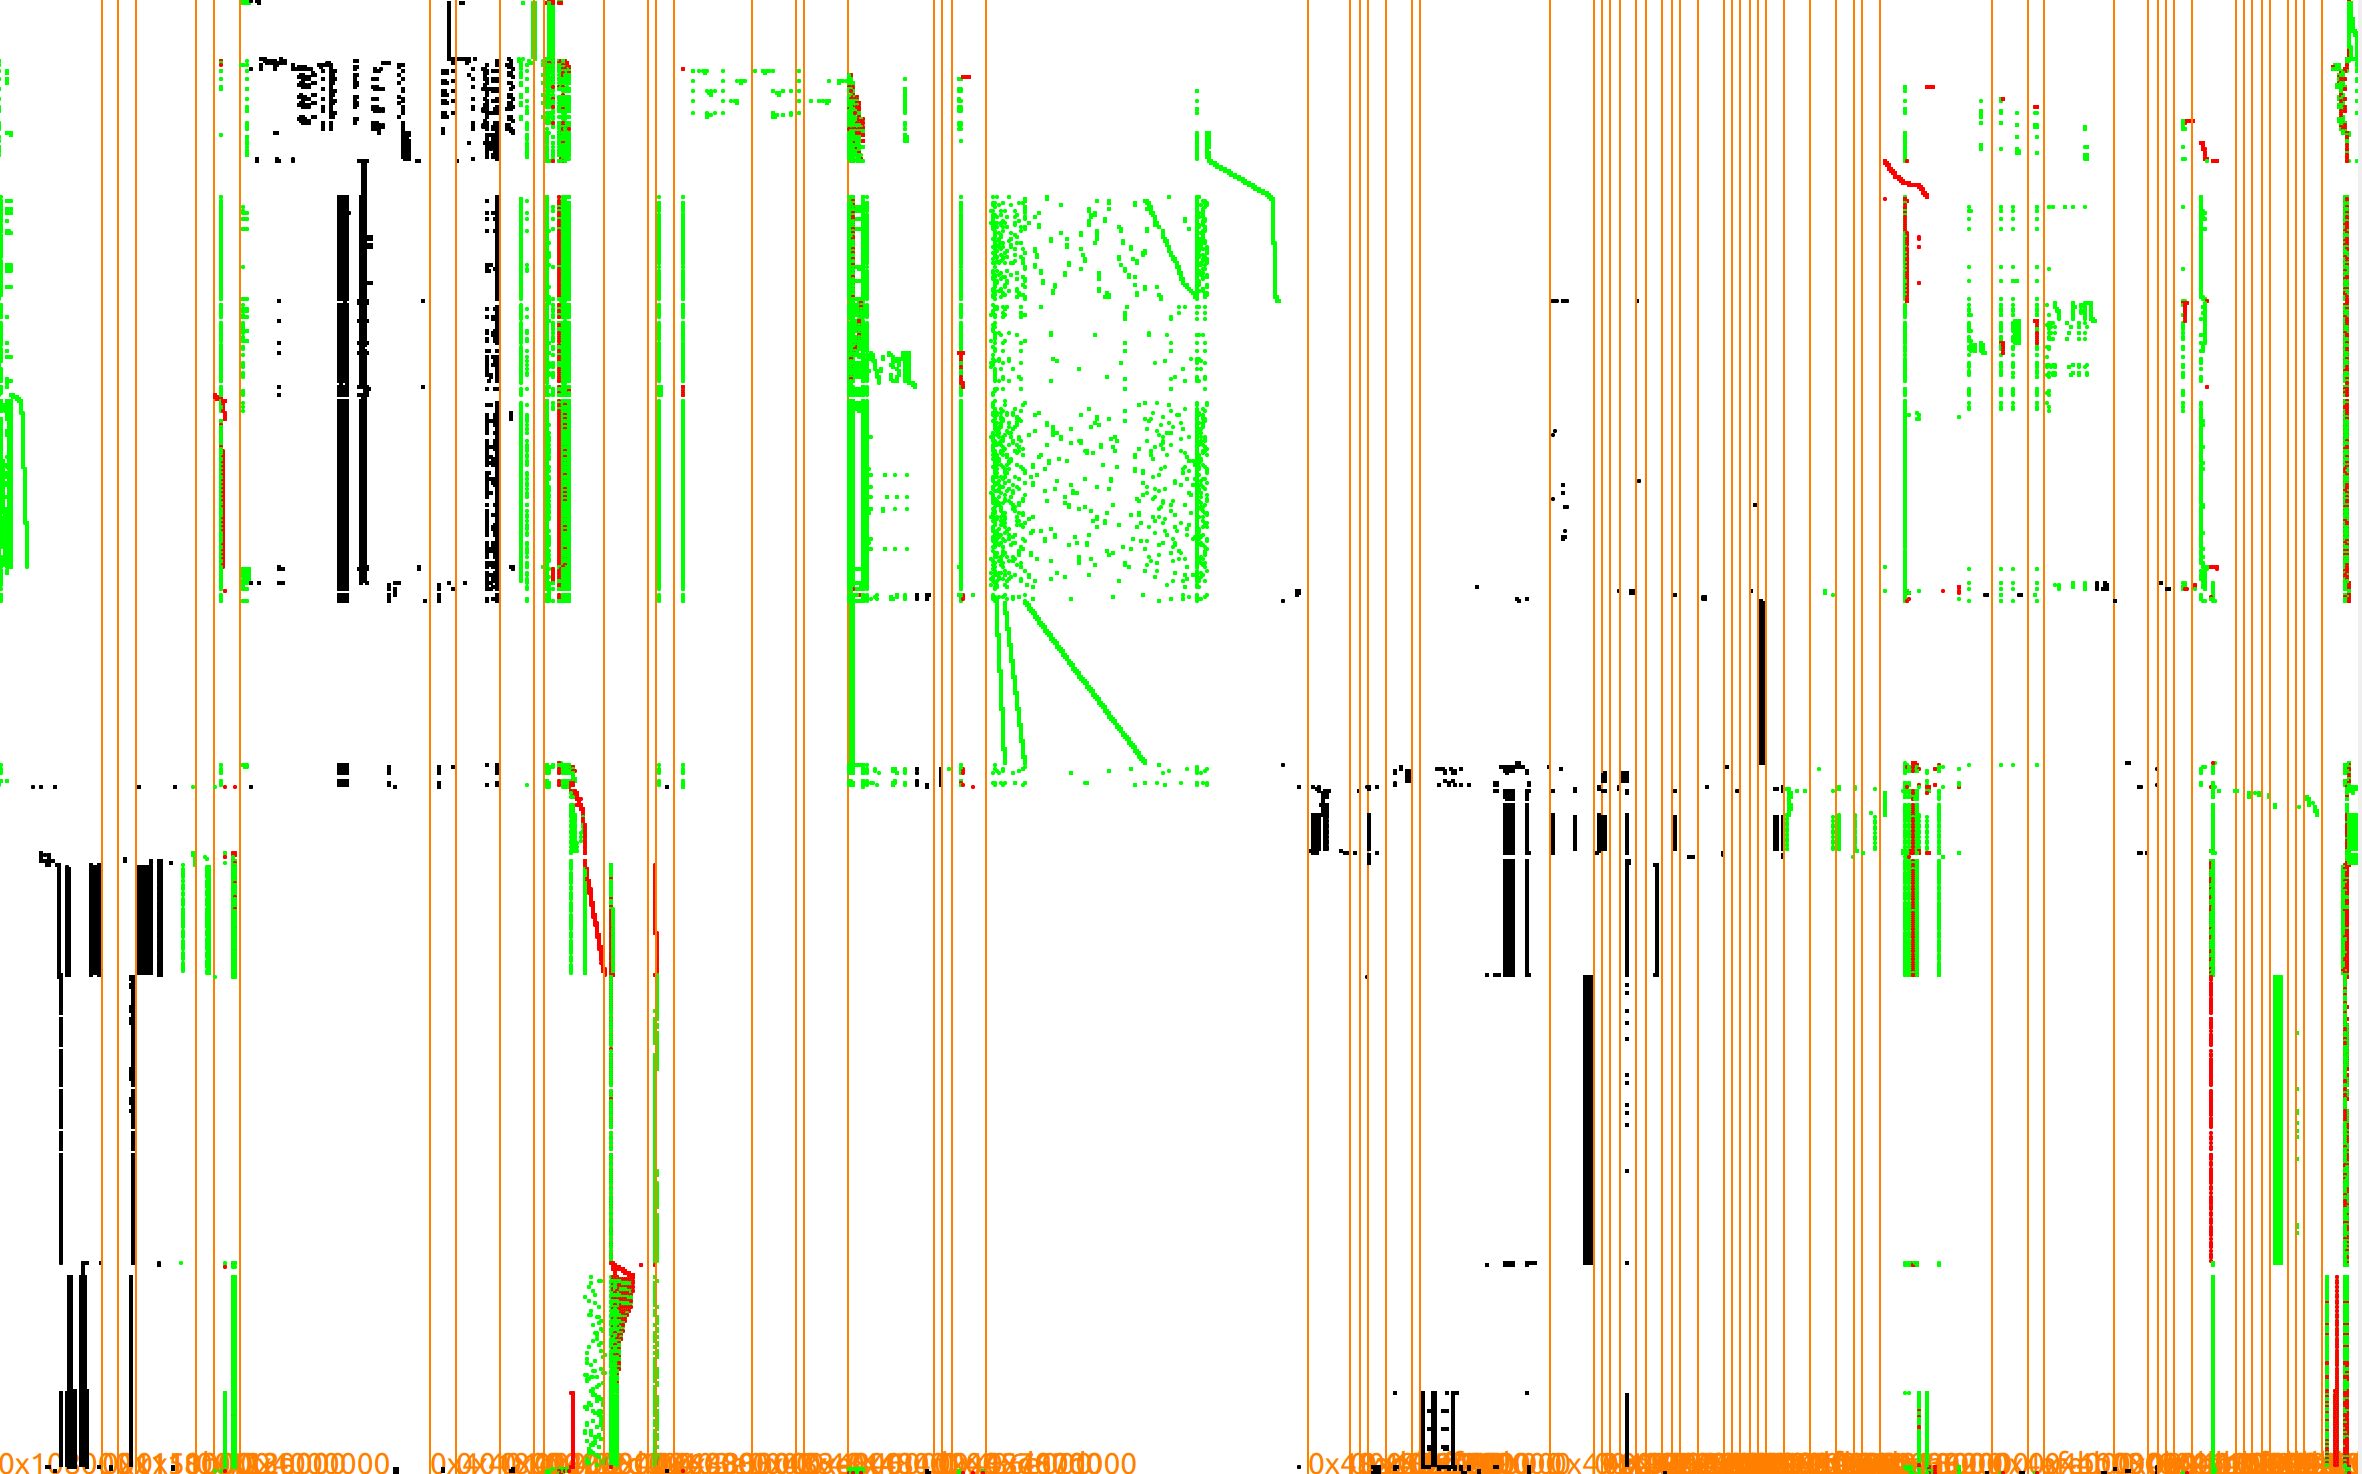
\includegraphics[scale=0.15]{Images/trace_ls.png}\\
L'abscisse représente les adresses mémoires et l'ordonnée le temps (de haut en bas). Un point vert correspond à une lecture en mémoire, un point rouge à une écriture en mémoire et un point noir à l'exécution d'une instruction.
\end{center}

\subsection{Le dépôt Daredevil}
Le dépôt Daredevil contient le programme source permettant d'effectuer la CPA (Correlation Power Analysis) sur des traces stockées sous une forme particulière. Ce programme ne fait pas la différence entre des traces de la consommation d'énergie d'un matériel physique et des traces mémoire d'une exécution logiciel c'est pourquoi le format des données doit être particulier.\\
Le programme prend en entrée un fichier de configuration dont la syntaxe est décrite dans le dépôt. Je souhaite quand même préciser certaines choses : 

\subsubsection{Les samples}
On considère qu'une trace est composée de "samples", ces samples représentent une donnée dans la trace. Par exemple pour une trace mémoire, un sample peut être une lecture, une écriture ou bien une exécution d'une instruction. La variable $index$ dans le fichier de configuration va permettre de dire à Daredevil à partir de quel sample des traces il doit commencer à analyser les données. La variable $nsamples$ permet de dire à Daredevil le nombre de sample qu'il doit analyser à partir d'$index$. L'intérêt que ces variables ont à être précisé est qu'on restreint la quantité de travail pour avoir une meilleure précision (par exemple ne cibler que le premier tour de l'AES). On aura donc une CPA plus rapide.

\subsubsection{La position}
Pour effectuer la CPA, Daredevil a besoin des messages d'entrées qu'on a utilisés pour générer les traces. À partir de ces derniers, Daredevil va construire les "guesses" : Daredevil va appliquer un ou exclusif, octets par octets, entre ces guesses et toutes les clés possibles puis appliquer une transformation grâce aux Lookup Table (LUT). Ainsi pour l'AES il aura simulé la première partie du premier tour pour tous les octets de clé possibles. Il calculera ensuite la corrélation entre la moyenne de ces résultats et la moyenne des données contenues dans chaque traces grâce au coefficient de Pearson. Un coefficient de corrélation sera affecté pour chaque octets de clé et celui ayant un coefficient plus élevé que les autres sera susceptible d'être un octet correct de la clé.\\
La position dans le fichier de configuration permet de préciser la position dans l'AES qu'on veut attaquer. Les deux positions qui m'ont étés les plus utiles sont $AES\_AFTER\_MULTINV$ et $AES\_AFTER\_SBOX$.

\subsubsection{L'ordre et window}
Daredevil offre la possibilité de faire une attaque d'ordre 1 et d'ordre 2. L'attaque d'ordre 1 est destinée aux implémentations n'utilisant pas de masquage.\\
\textbf{Rappel du masquage : }Le masquage permet de décomposer les variables sensible de l'algorithme (ici la clé) en plusieurs variables qu'on appelle masques. On va dérouler l'algorithme en utilisant ces masques. Certaines opérations de l'algorithme doivent être donc adaptées pour que le chiffré final reste le même. On dira qu'un masquage d'ordre 1 est la décomposition de la clé en 2 variables, un masquage d'ordre 2 est la décomposition de la clé en 3 variables, etc... L'intérêt du masquage est de modifier les valeurs intermédiaires et ainsi rendre la DPA et la CPA d'ordre 1 inefficace.\\
La CPA d'ordre 2 permet de casser les implémentations utilisant un masquage d'ordre 1. Daredevil va combiner chaque paires de samples (leur valeurs ayant été soustraite par la moyenne des traces) compris dans un certain intervalle (en terme de sample) lors du calcul de la corrélation. Cet intervalle est appelé "window" et est à préciser dans le fichier de configuration pour une CPA d'ordre supérieur à 1.\\
\textbf{Exemple : }Si on a au total dans une trace 20 samples, qu'on souhaite effectuer l'attaque seulement sur 10 samples à partir du 5ème, qu'on souhaite faire une CPA d'ordre 2 et que l'intervalle dans lequel on veut qu'il teste toutes les paires possible soit d'une taille de 3, on aura :
\begin{itemize}
\item index=4
\item nsamples=10
\item order=2
\item window=3
\end{itemize}


\subsection{Le dépôt Deadpool}
Le dépôt Deadpool de Side-Channel Marvels propose un script Python $deadpool\_dca.py$ très utile permettant d'automatiser l'enregistrement de plusieurs traces et de convertir ces enregistrement en fichier exploitable par Daredevil. Il contient également un certain nombre d'attaques DCA complètes et détaillées (qui ont étés utiles pour moi pour m'entrainer).\\
Le fichier $deadpool\_dca.py$ détaille déjà bien comment l'utiliser cependant je souhaite quand même présenter son utilisation. Voici le script typique me permettant de générer des traces :\\

\lstinputlisting{Images/enregistrement_traces.py}

Ici on appelle le constructeur de la classe $TracerGrind$ qui comprend plusieurs paramètres (certains sont optionnels) :
\begin{itemize}
\item Le nom de l'exécutable sur lequel on va enregistrer les traces
\item Une fonction permettant de savoir la forme de ce que l'exécutable attend en entrée
\item Une fonction permettent de savoir la forme de ce que l'exécutable donne en sortie
\item L'architecture de la machine
\item La taille d'un bloc (ici 16, c'est à dire 16 blocs de 8 bits = 128 correspondant à l'AES-128 bits)
\item L'intervalle en terme d'adresse qu'on veut enregistrer
\item L'intervalle en terme d'adresse de la pile
\end{itemize}
Suite à cela, on appelle la méthode $run$ en précisant le nombre de traces qu'on veut enregistrer (ici 1000). Et pour finir, on appelle la fonction $bin2daredevil$ qui transforme les traces enregistrées en fichiers que le programme daredevil accepte pour faire une CPA. Ici on précise qu'on veut que cette fonction produise un fichier de configuration faisant l'attaque à la position après la S-Box et l'autre à la position après la multiplication inverse.\\\\
Ce script produit alors, si tout s'est bien passé :
\begin{itemize}
\item Des fichiers $.input$ et $.output$ contenants respectivement les entrées données à l'exécutable et les sorties renvoyées par l'exécutable dans l'ordre. Plusieurs fichiers de la sorte sont générés, seul le nom diffère (utile pour Daredevil).
\item Des fichiers $.trace$ contenants les données des traces. Par défaut, on aura les fichiers commençants par $mem\_data$ permettant de faire l'attaque sur les données contenues dans les différentes adresses, les fichiers commençants par $mem\_addr1$ permettant de faire l'attaque sur la valeur des adresses, et les fichiers commençants par $stack$ permettant de faire l'attaque sur les données contenues dans la pile.
\item Des fichiers $.config$ contenants toutes les informations nécessaires pour lancer une CPA avec Daredevil. Ces fichiers sont à donner en entrée au programme daredevil. Deadpool ne permet pas de générer des fichiers de configuration pour une attaque d'ordre 2, il est donc nécessaire de modifier/créer soit même un fichier de configuration pour faire ce type d'attaque.
\end{itemize}


\section{Mes différentes attaques}
\subsection{Implémentation basique de l'AES-128}
J'ai pu récupérer une implémentation basique de l'AES-128 (sans protection contre les attaques en boîte blanche) sur ce lien : \href{https://github.com/dhuertas/AES}{https://github.com/dhuertas/AES}.\\\\
Tout d'abord on lance l'enregistrement complet d'une trace mémoire de l'exécution du programme. Voici une capture d'écran de ce qu'on obtient :

\begin{center}
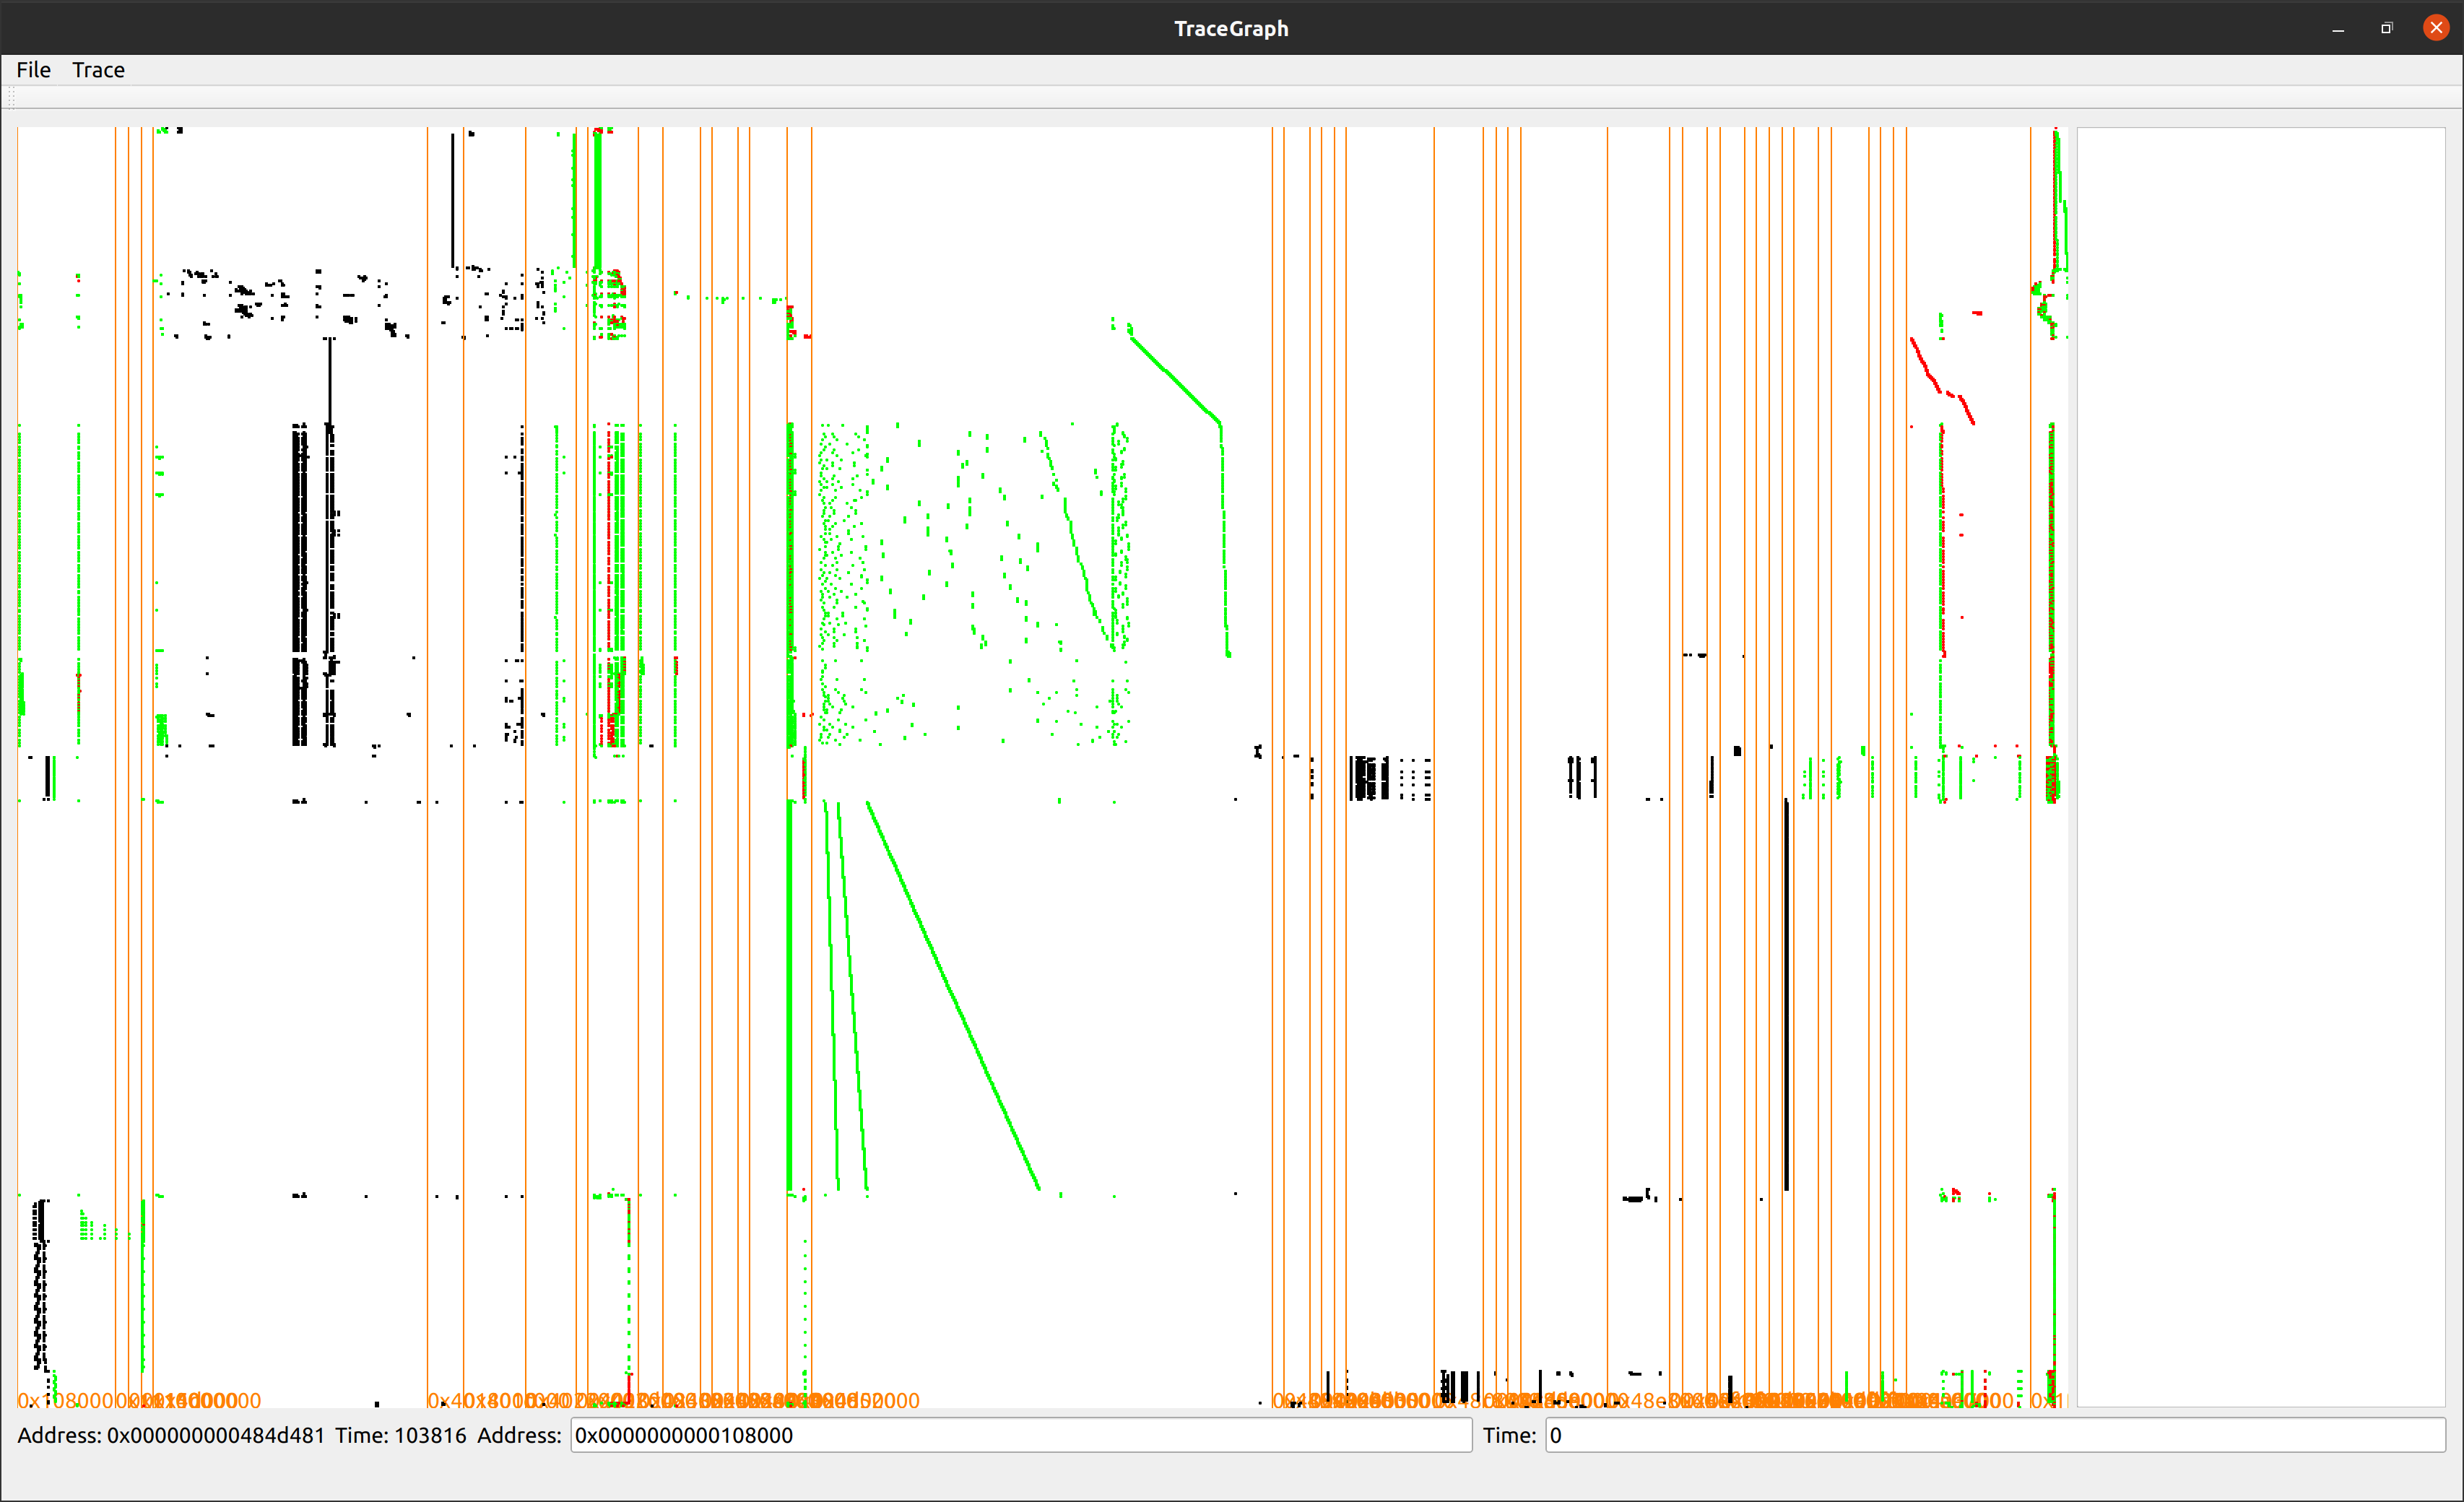
\includegraphics[scale=0.11]{Images/AES_basique_sans_filtre.png}\\
\end{center}
À priori il est assez difficile de distinguer un motif qui pourrait correspondre à l'AES. Cependant, lorsqu'on zoom et qu'on parcours un peu cette représentation graphique, on peut remarquer ceci :

\begin{center}
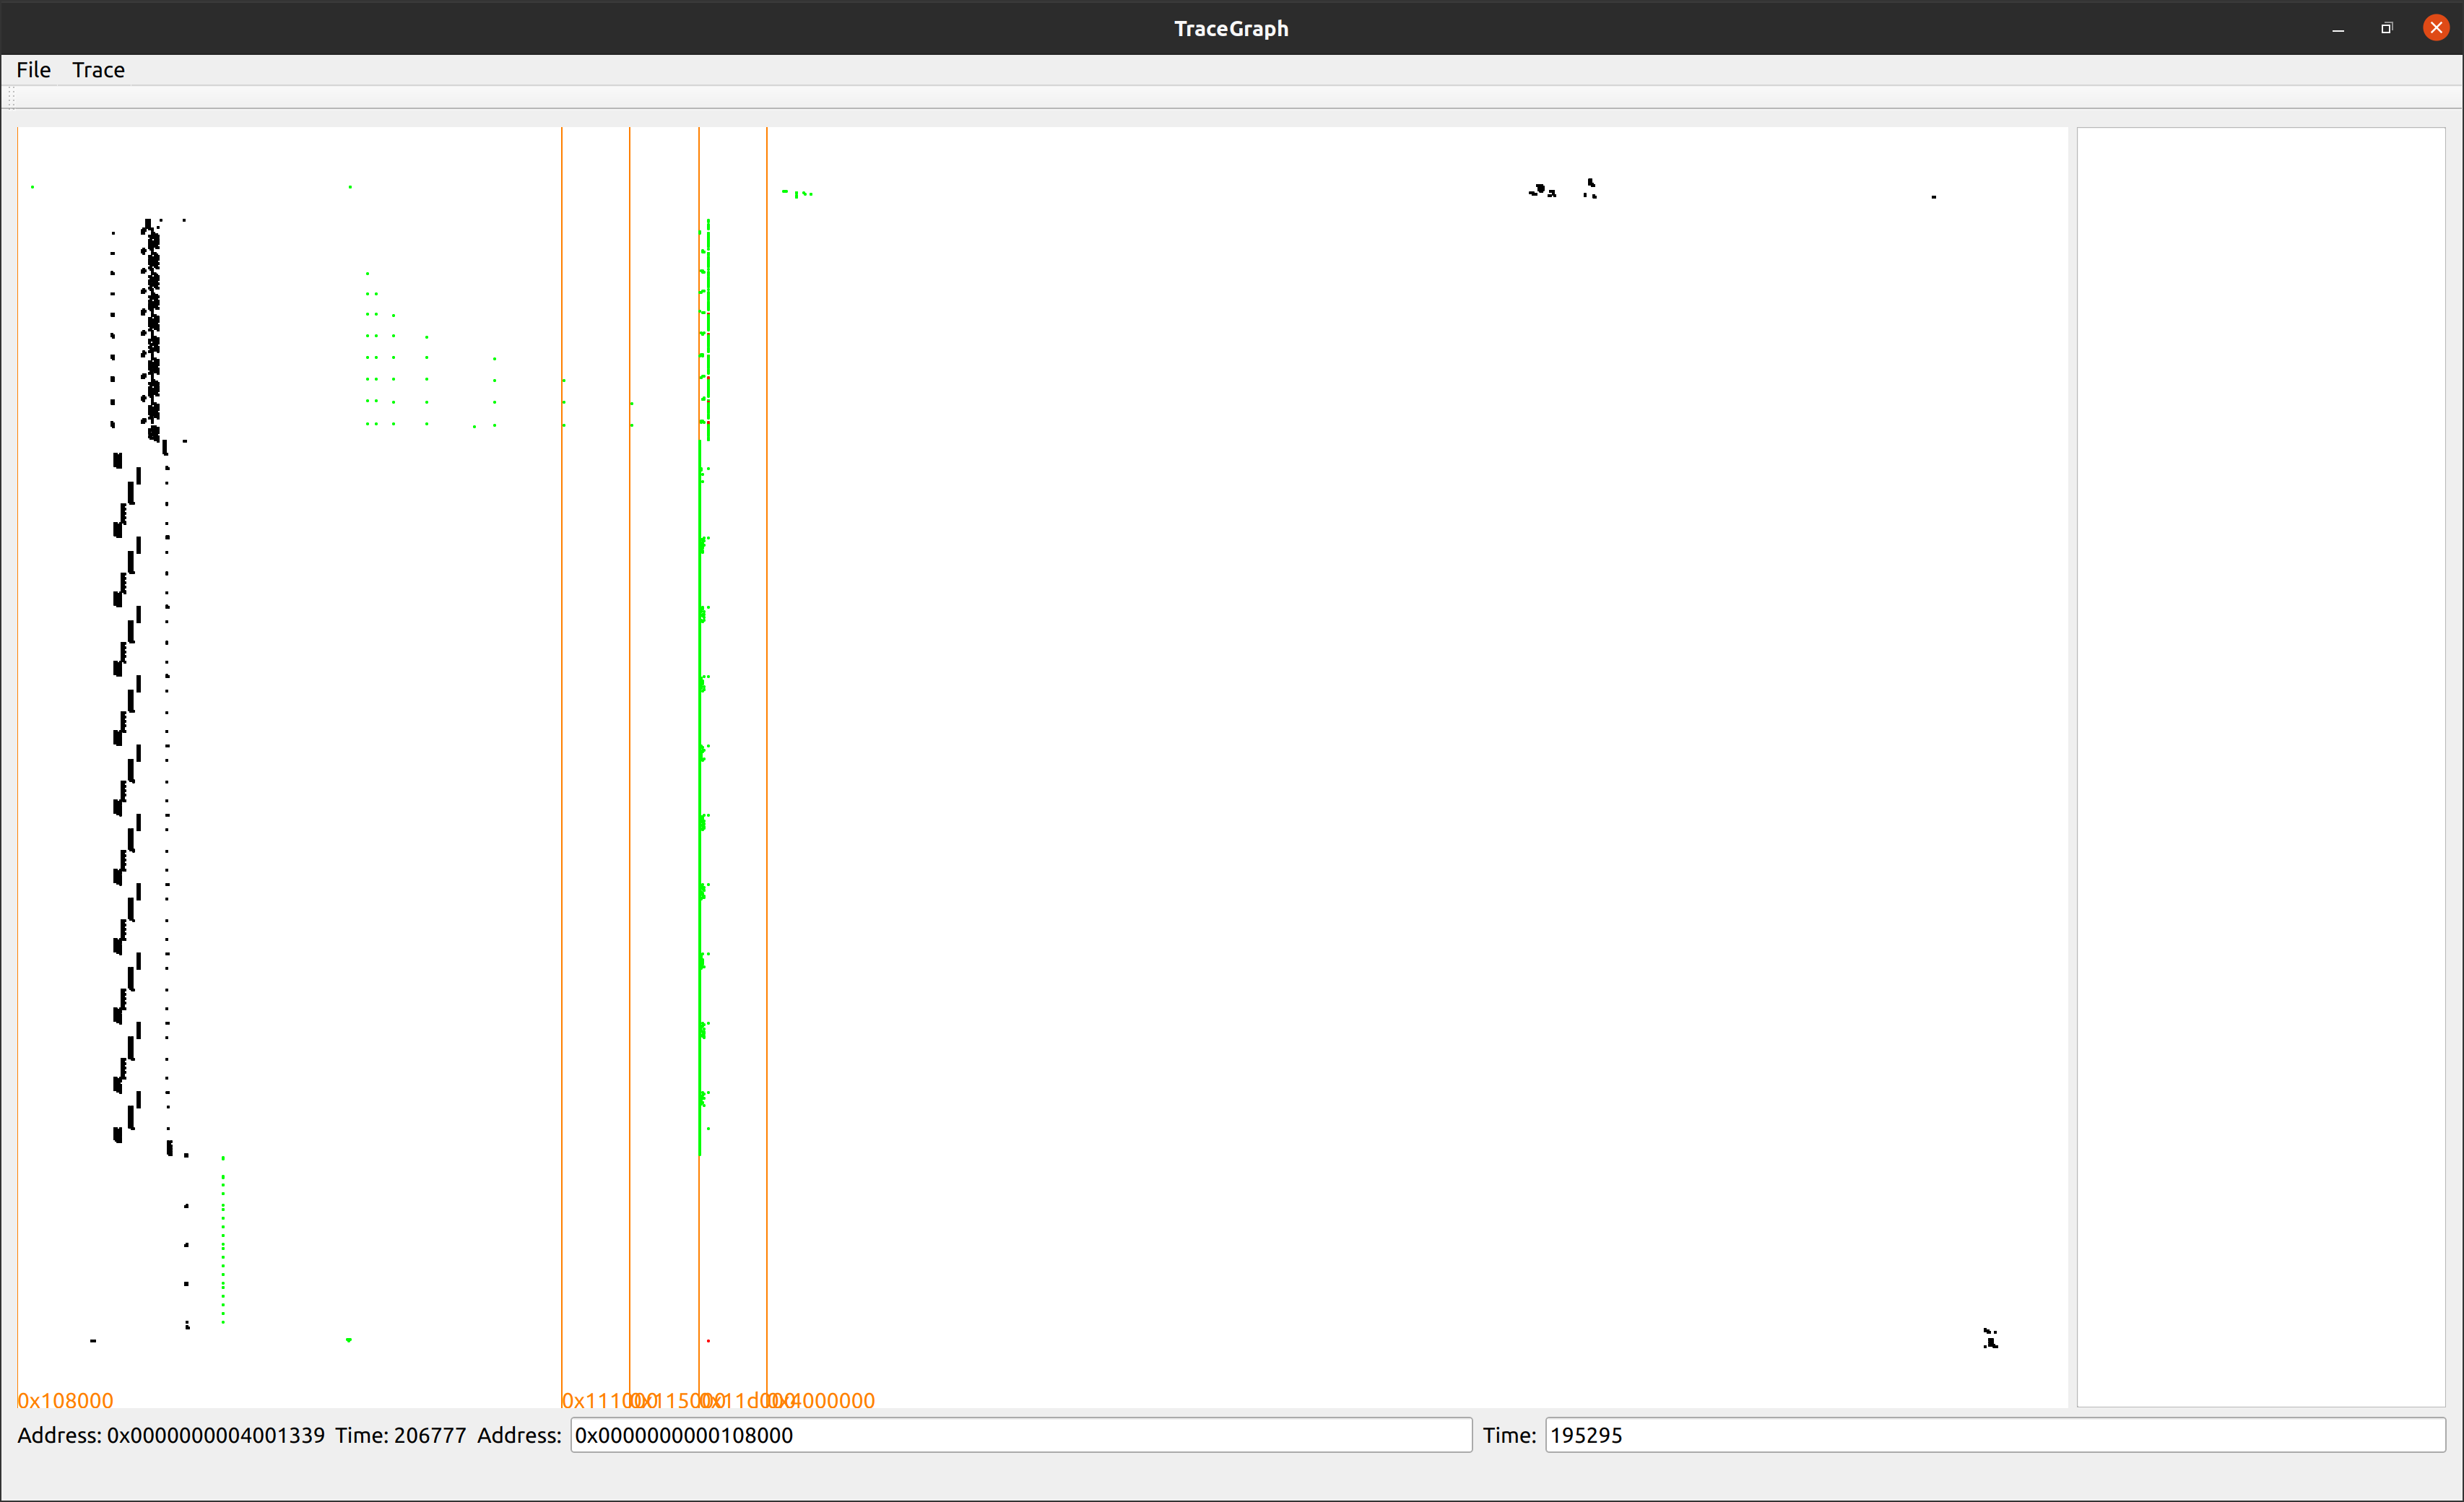
\includegraphics[scale=0.11]{Images/AES_basique_zoom.png}\\
\end{center}
Ici on voit clairement la répétition de 10 même motifs puis la répétition de 9 autres motifs + 1 plus petit à la fin. Cela pourrait vraiment correspondre à la génération des sous-clés et aux 10 tours de l'AES.\\
On relance alors un enregistrement avec cette fois ci un filtre : on ne garde que les intervalles sur lesquels on observe des lectures/écritures/instructions sur l'espace de temps des motifs qu'on vient de remarquer. Ici le filtre qu'on pose est :

\begin{lstlisting}
"0x108000-4000000, 0x402d000-0x4830000, 0x484d000-0x4852000"
\end{lstlisting}
Voici ce que nous obtenons :

\begin{center}
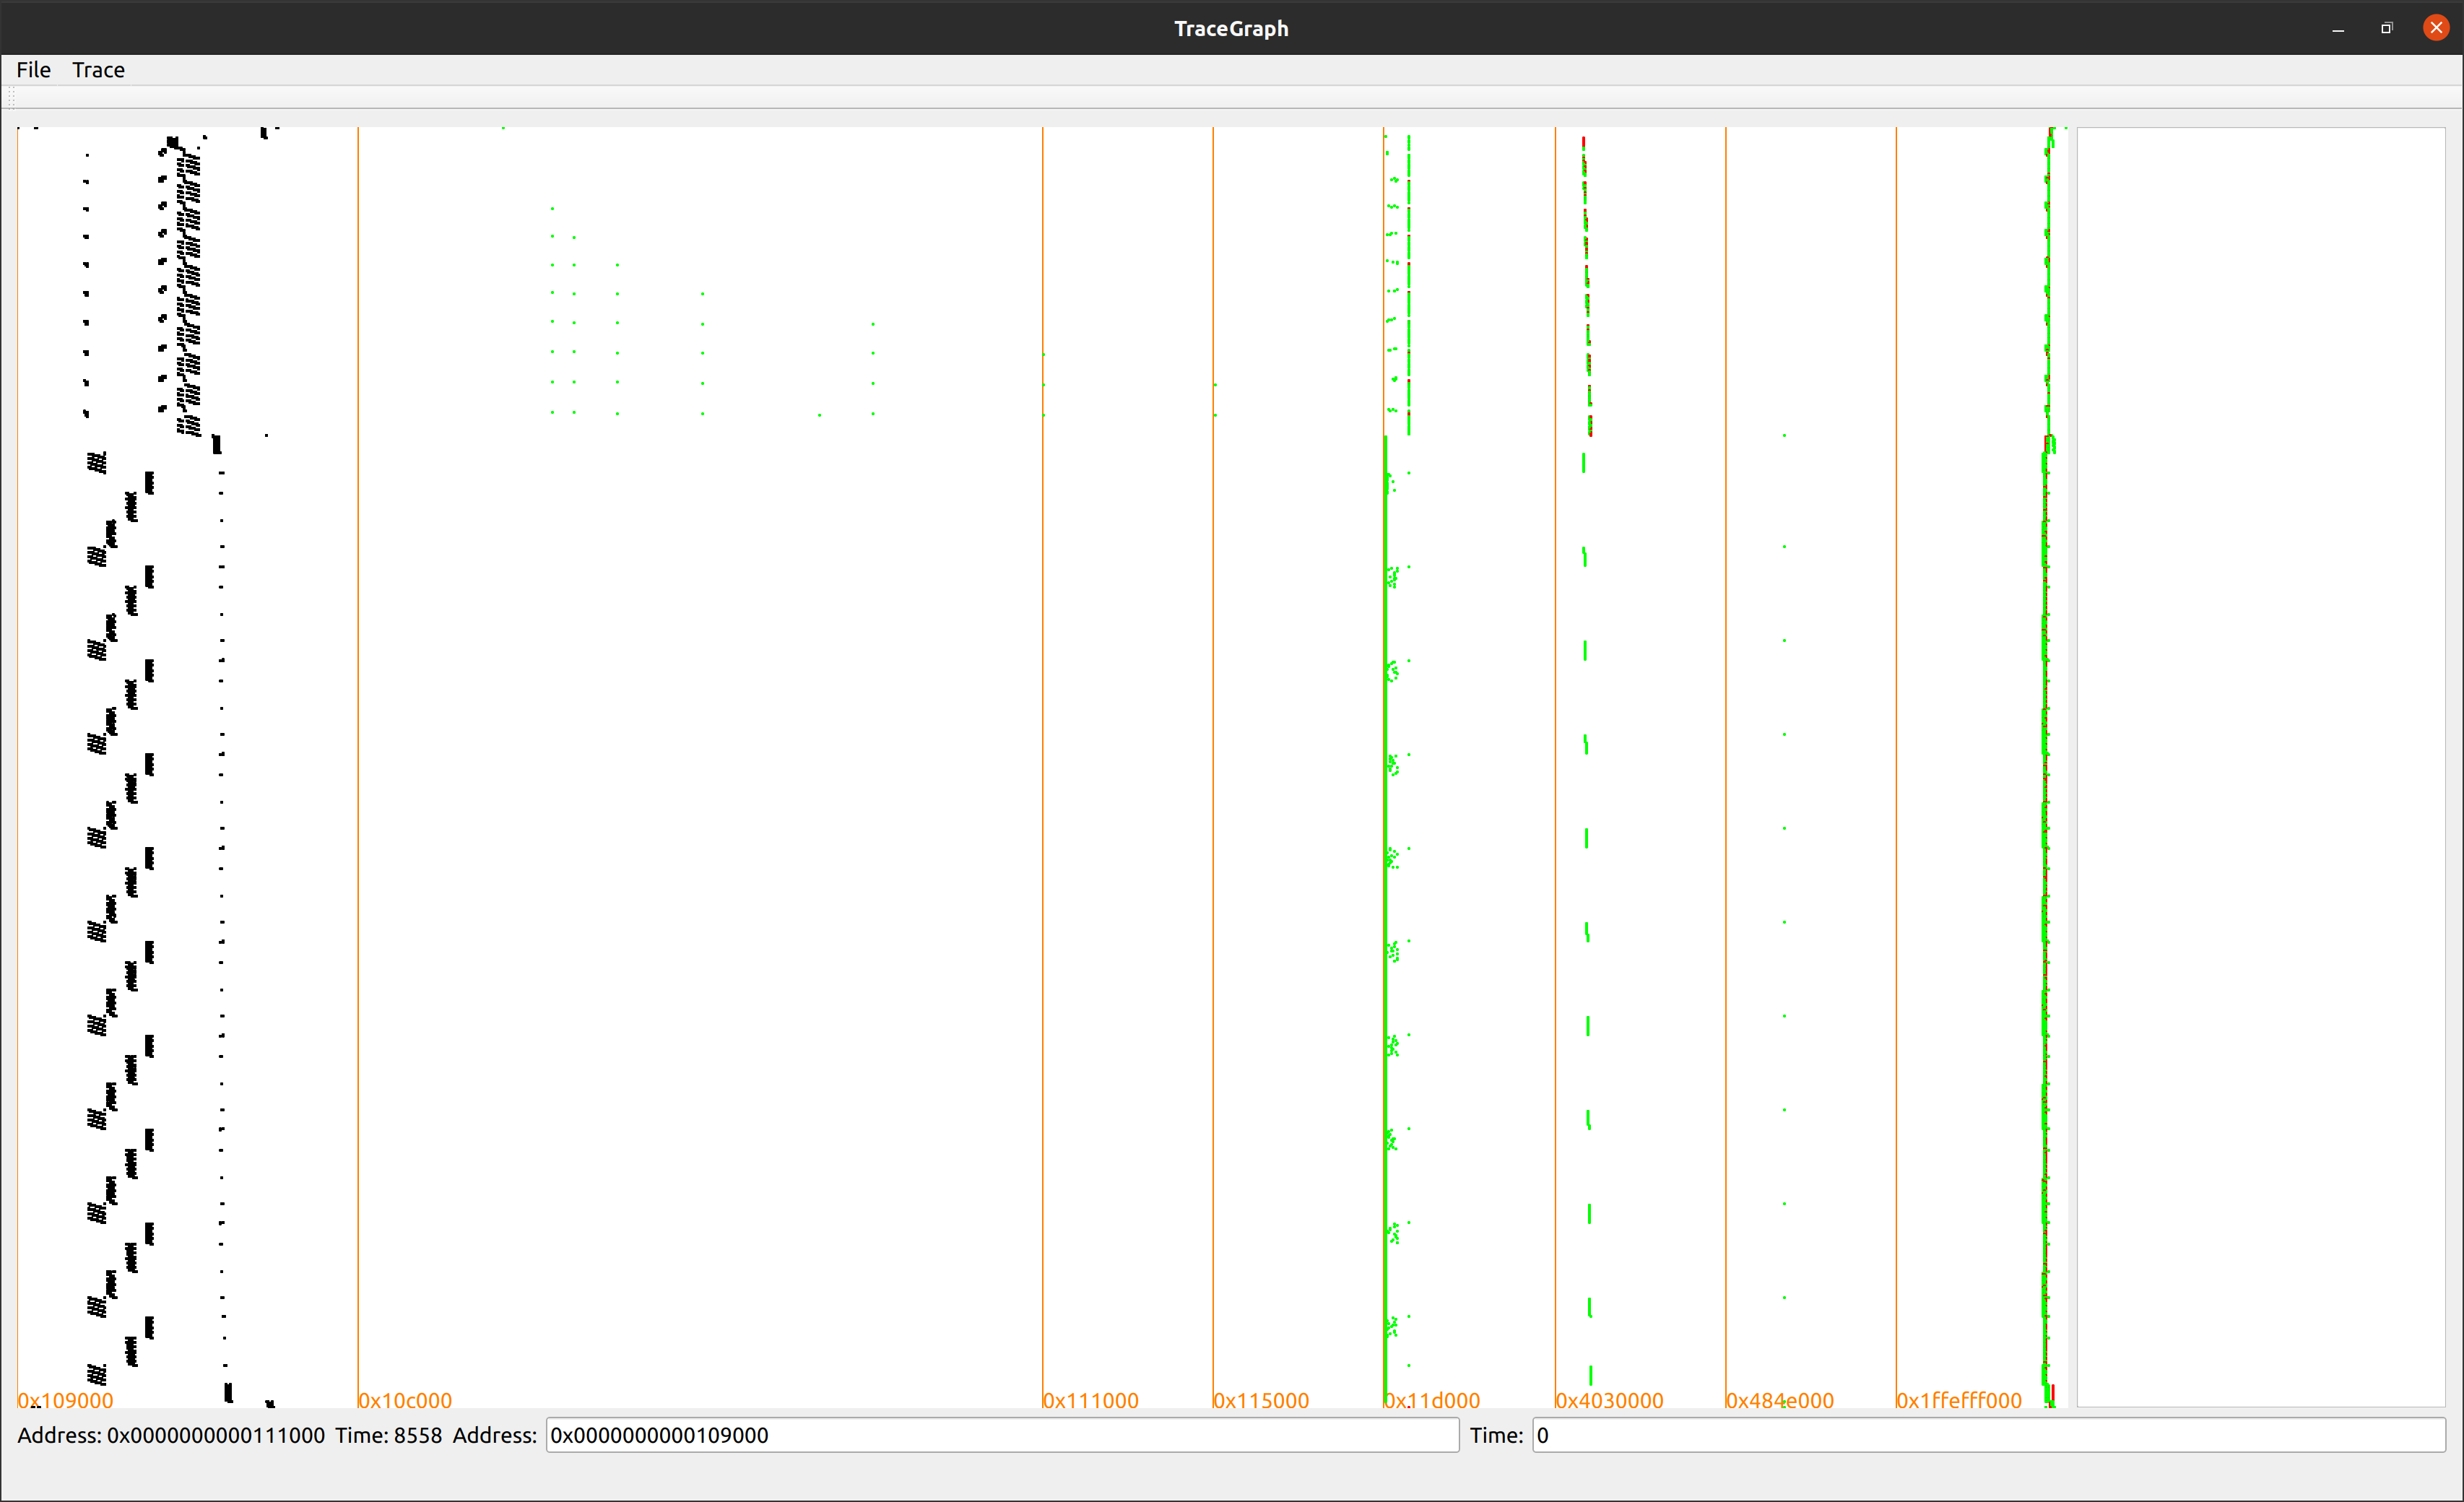
\includegraphics[scale=0.11]{Images/AES_basique_filtre.png}\\
\end{center}
Cela correspond à ce que nous cherchons. On observe également que la trace comprend bien la pile (tout à droite).\\
On lance maintenant l'enregistrement de 30 traces avec deadpool pour commencer puis on effectue une CPA avec daredevil avec le fichier de configuration utilisant les données et ayant pour position $AES\_AFTER\_MULTINV$.
Voici ce qu'on obtient dans le terminal pour le premier octet :

\begin{center}
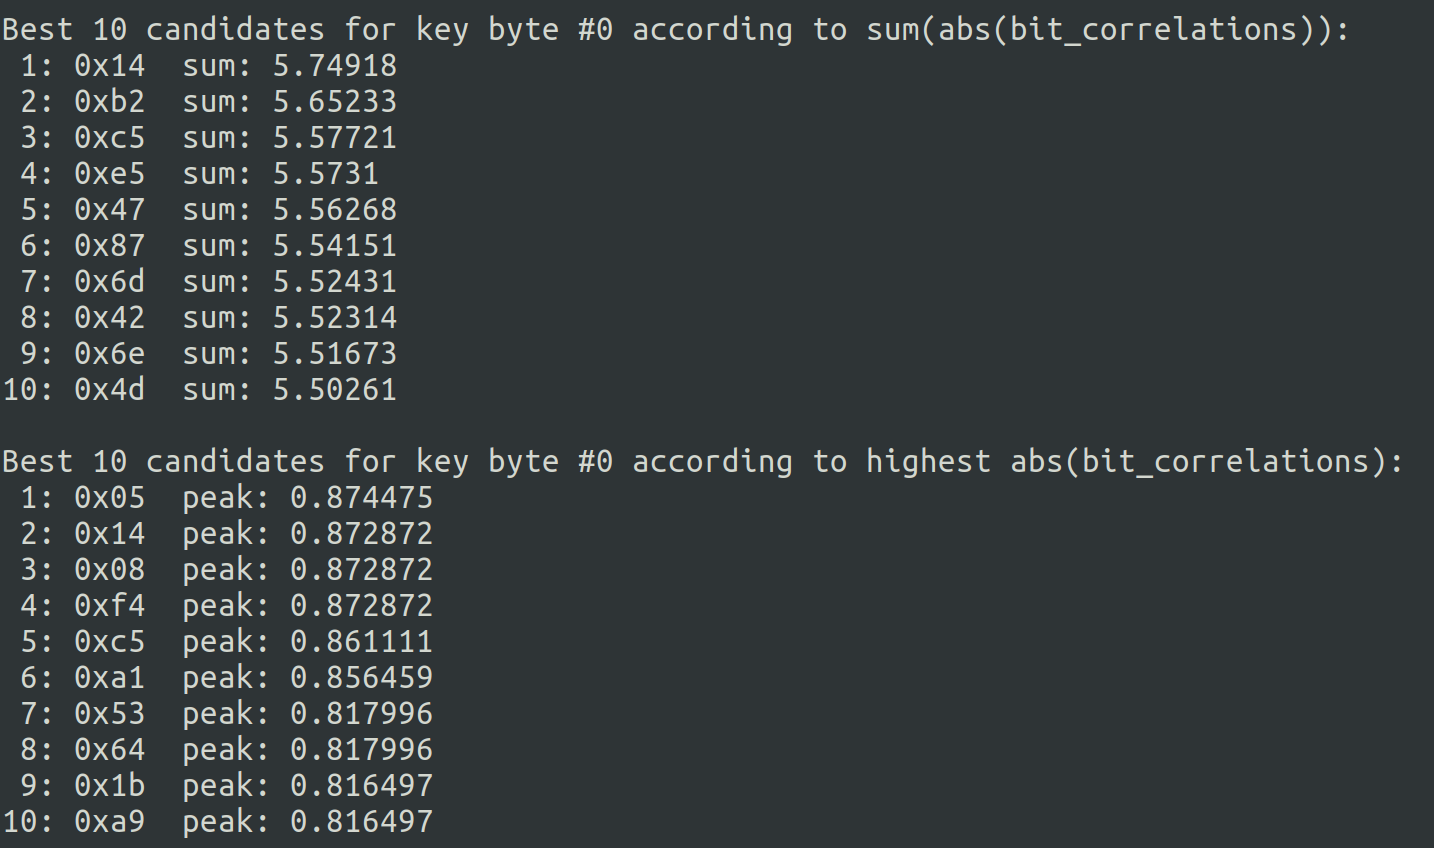
\includegraphics[scale=0.25]{Images/Resultat_AES_basique_echec}\\
\end{center}
Ici on n'observe pas de coefficient de corrélation se démarquant particulièrement des autres (l'écart entre le premier plus élevé et le deuxième plus élevé est assez faible). On obtient un résultat similaire pour tous les autres octets et donc on ne peut pas en déduire la clé.\\
On essaye alors la même chose mais en utilisant le fichier de configuration ayant pour position $AES\_AFTER\_SBOX$ et voici ce qu'on obtient pour le premier octet :

\begin{center}
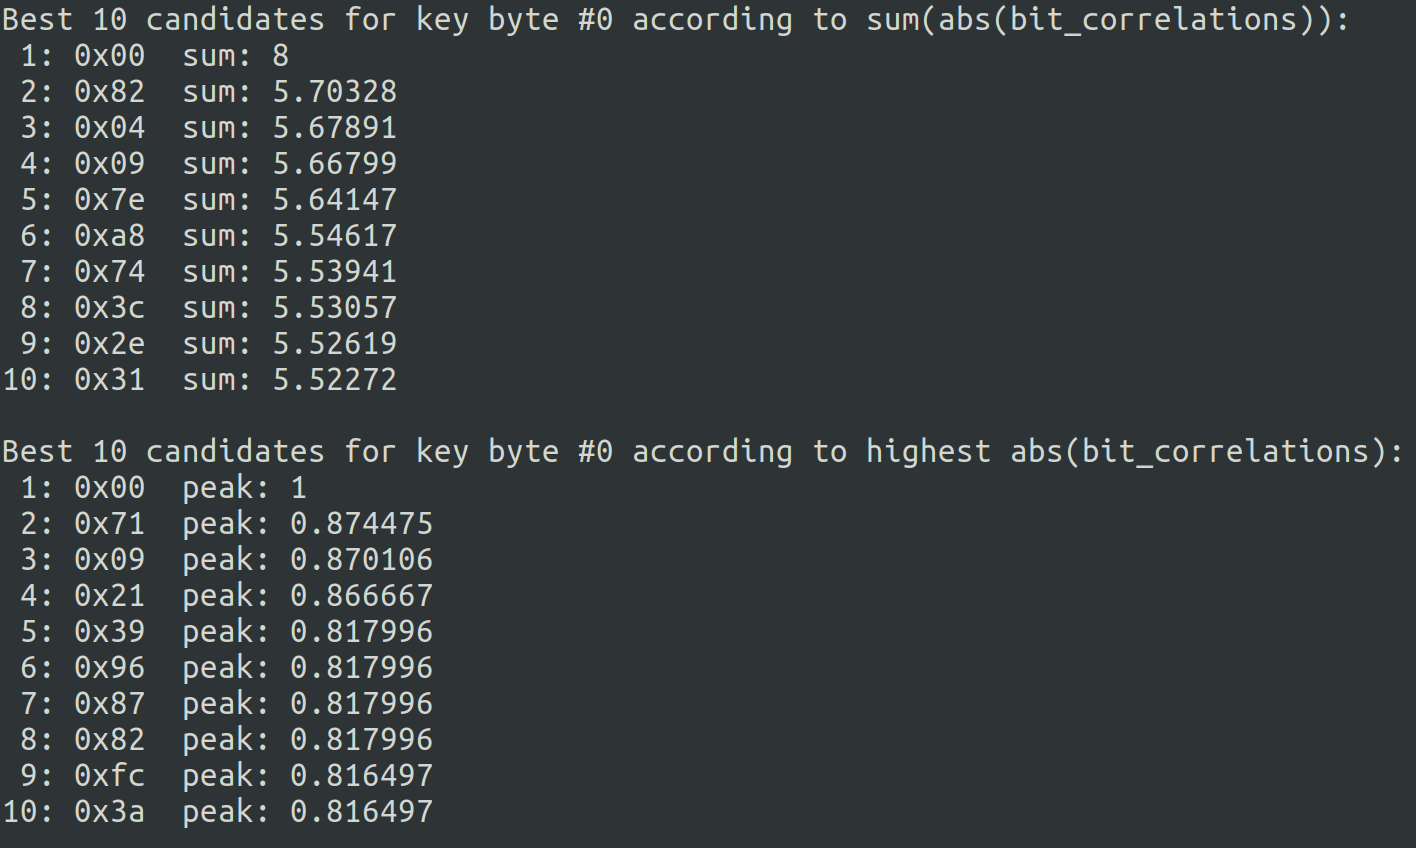
\includegraphics[scale=0.25]{Images/Resultat_AES_basique_succes}\\
\end{center}
Ici on observe une réelle différence entre le coefficient le plus élevé et le deuxième plus élevé. On en déduit donc que cet octet pourrait vraiment correspondre au vrai premier octet de la clé. On obtient cela pour tous les octets et on peut donc en déduire la clé. Ici la clé obtenue était $000102030405060708090A0B0C0D0E0F$ (choisi par moi-même).

\subsection{WhibOx Contest}
Il est possible de trouver plusieurs implémentations en boîte blanche de l'AES-128 sur le site \href{https://whibox-contest.github.io}{https://whibox-contest.github.io}. J'y suis donc allé pour essayer de casser des implémentations plus protégées qu'une implémentation basique.

\subsubsection{WhibOx Contest 2019 numéro 26}
Je me suis intéressé à l'implémentation 26 \textit{distracted$\_$leavitt} du WhibOx Contest de 2019.\\
Comme pour l'implémentation basique, on commence par générer une trace complète de l'exécution. Voici ce qu'on obtient :

\begin{center}
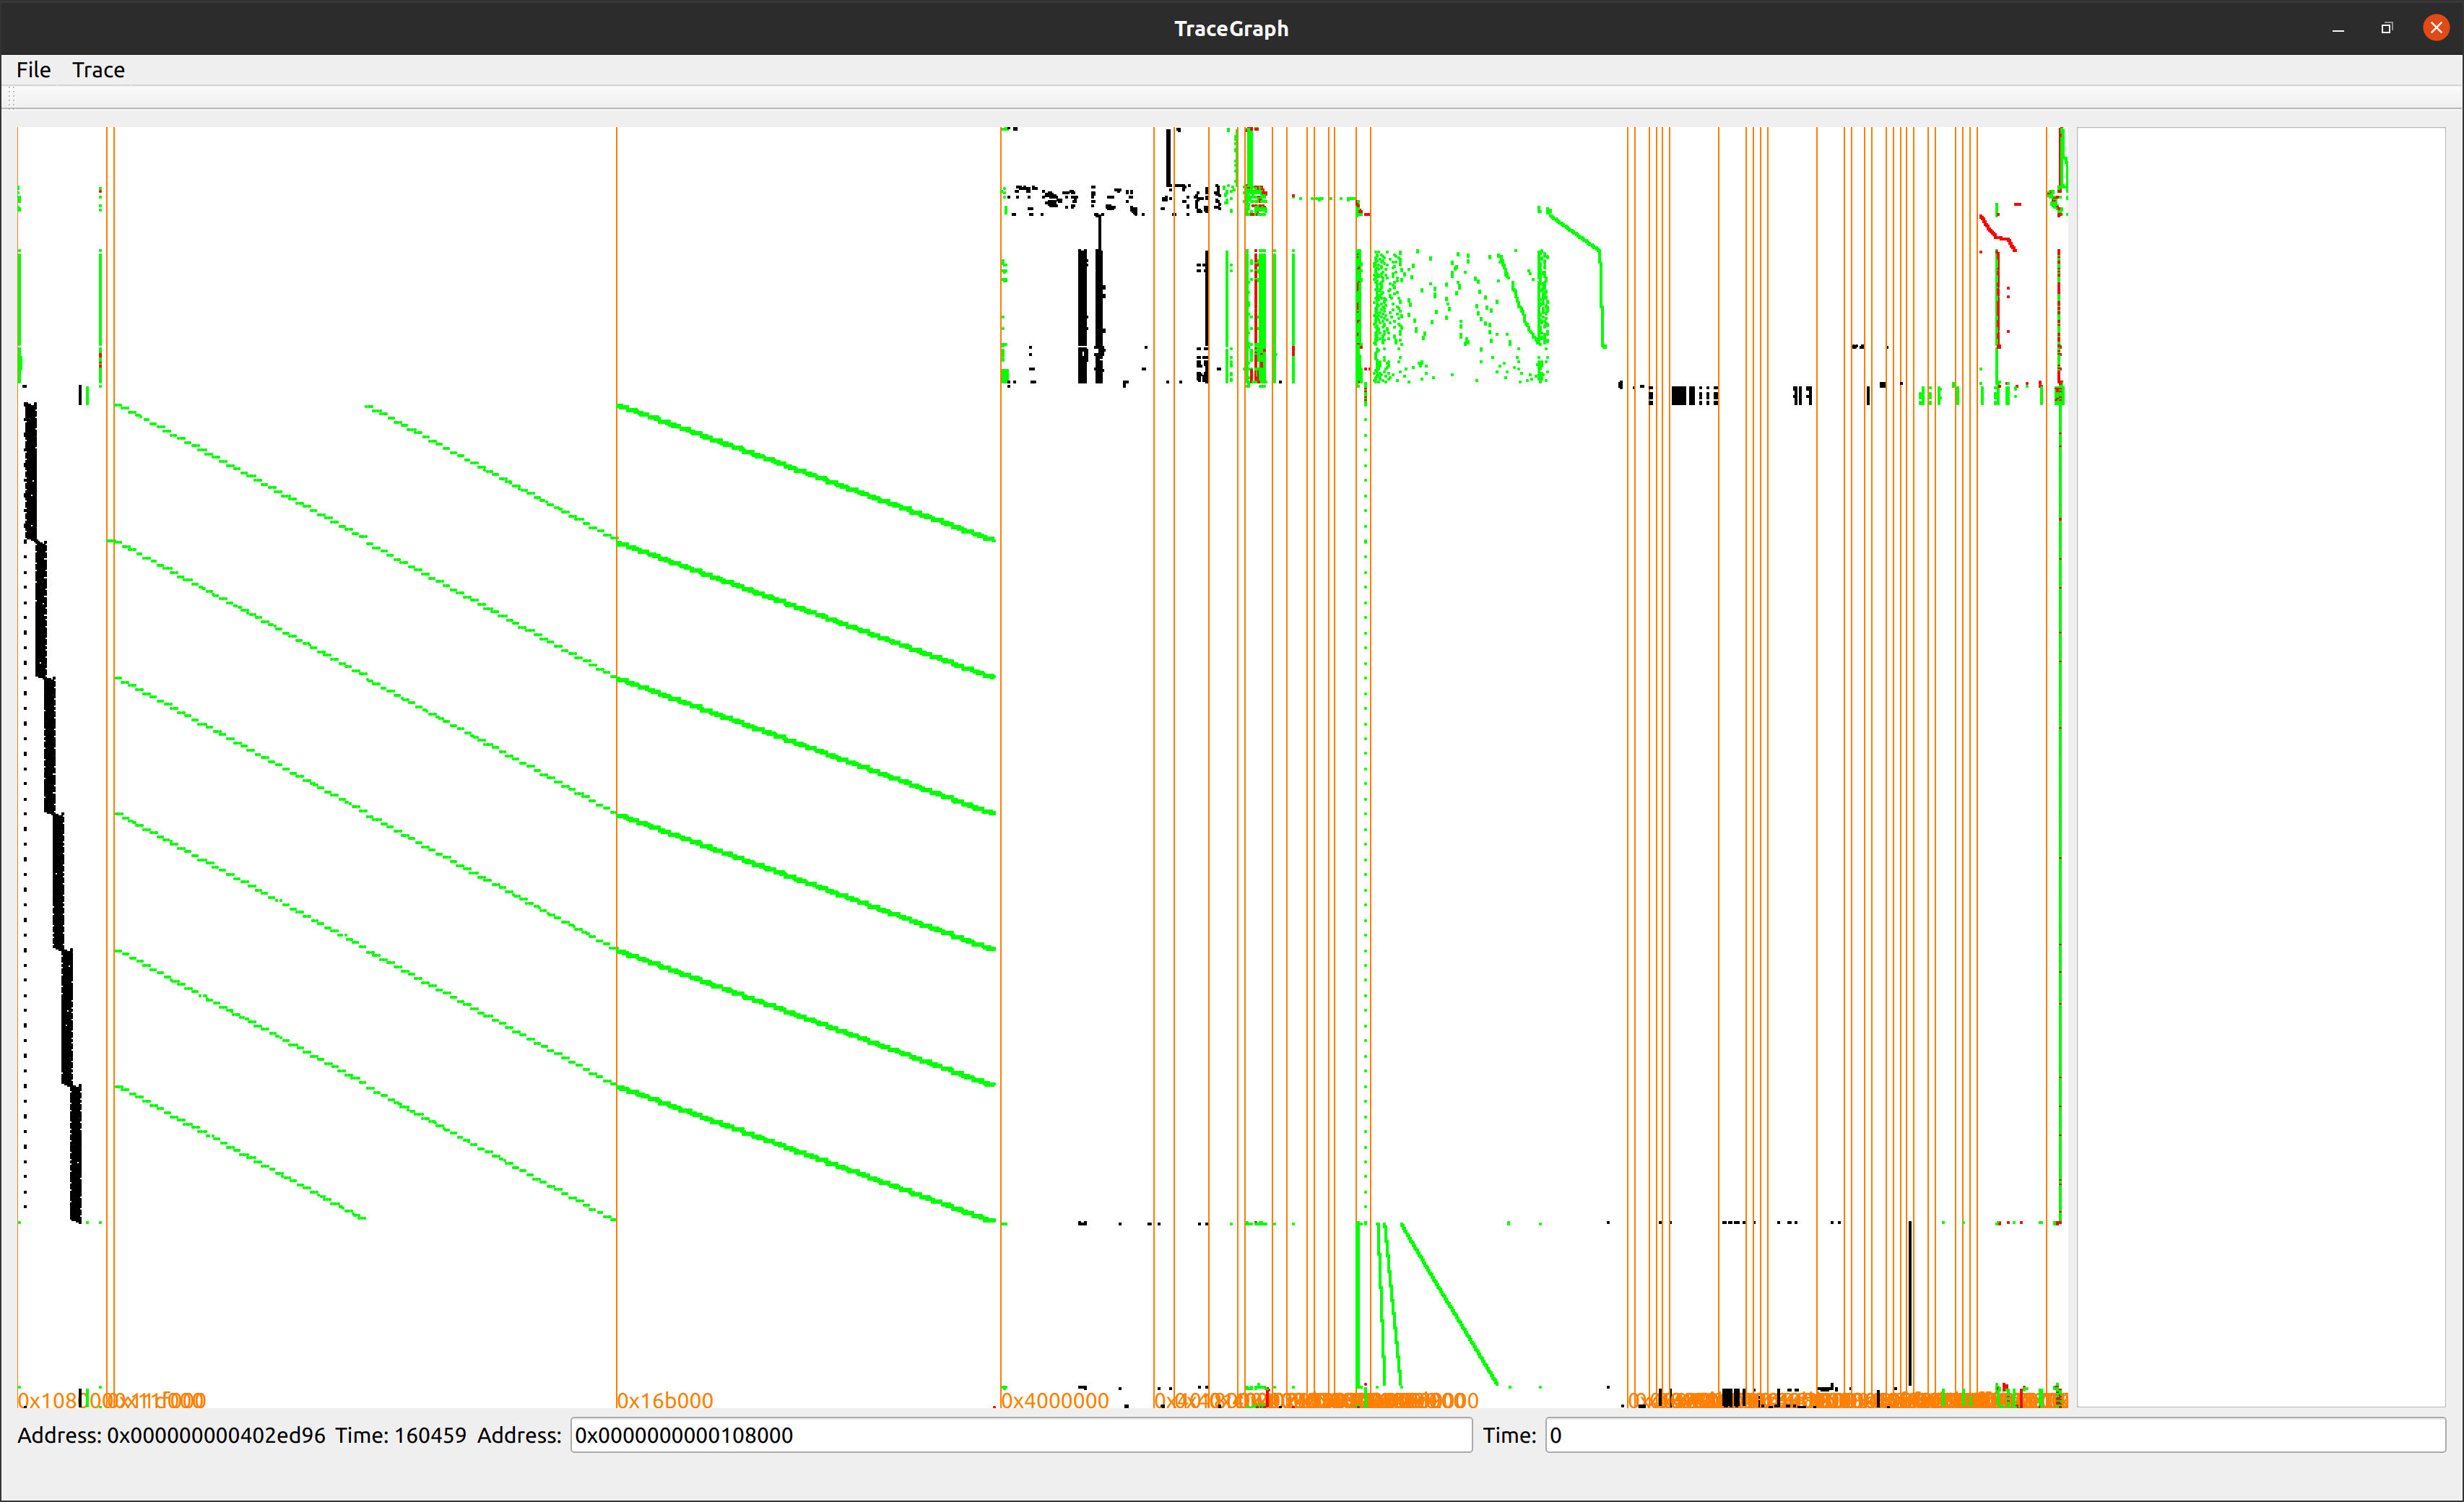
\includegraphics[scale=0.11]{Images/26_sans_filtre.png}\\
\end{center}
On remarque ici clairement un motif particulier entre l'adresse $0x108000$ et $0x4000000$. En noir (les instructions) on voit la répétition de 10 motifs qui pourrait correspondre à l'AES-128. On remarque cependant qu'en vert, la quantité de lecture est très importante mais ne ressemble pas à l'exécution d'un AES-128. Ceci à dû à la manière d'implémenter l'AES. En effet l'implémentation comporte la définition de grandes tables dans lesquelles l'algorithme va lire des données pour dérouler l'AES. Ces tables contiennent notamment la clé de manière dissimulé.\\
Voici maintenant ce qu'on obtient en appliquant le filtre adapté :

\begin{center}
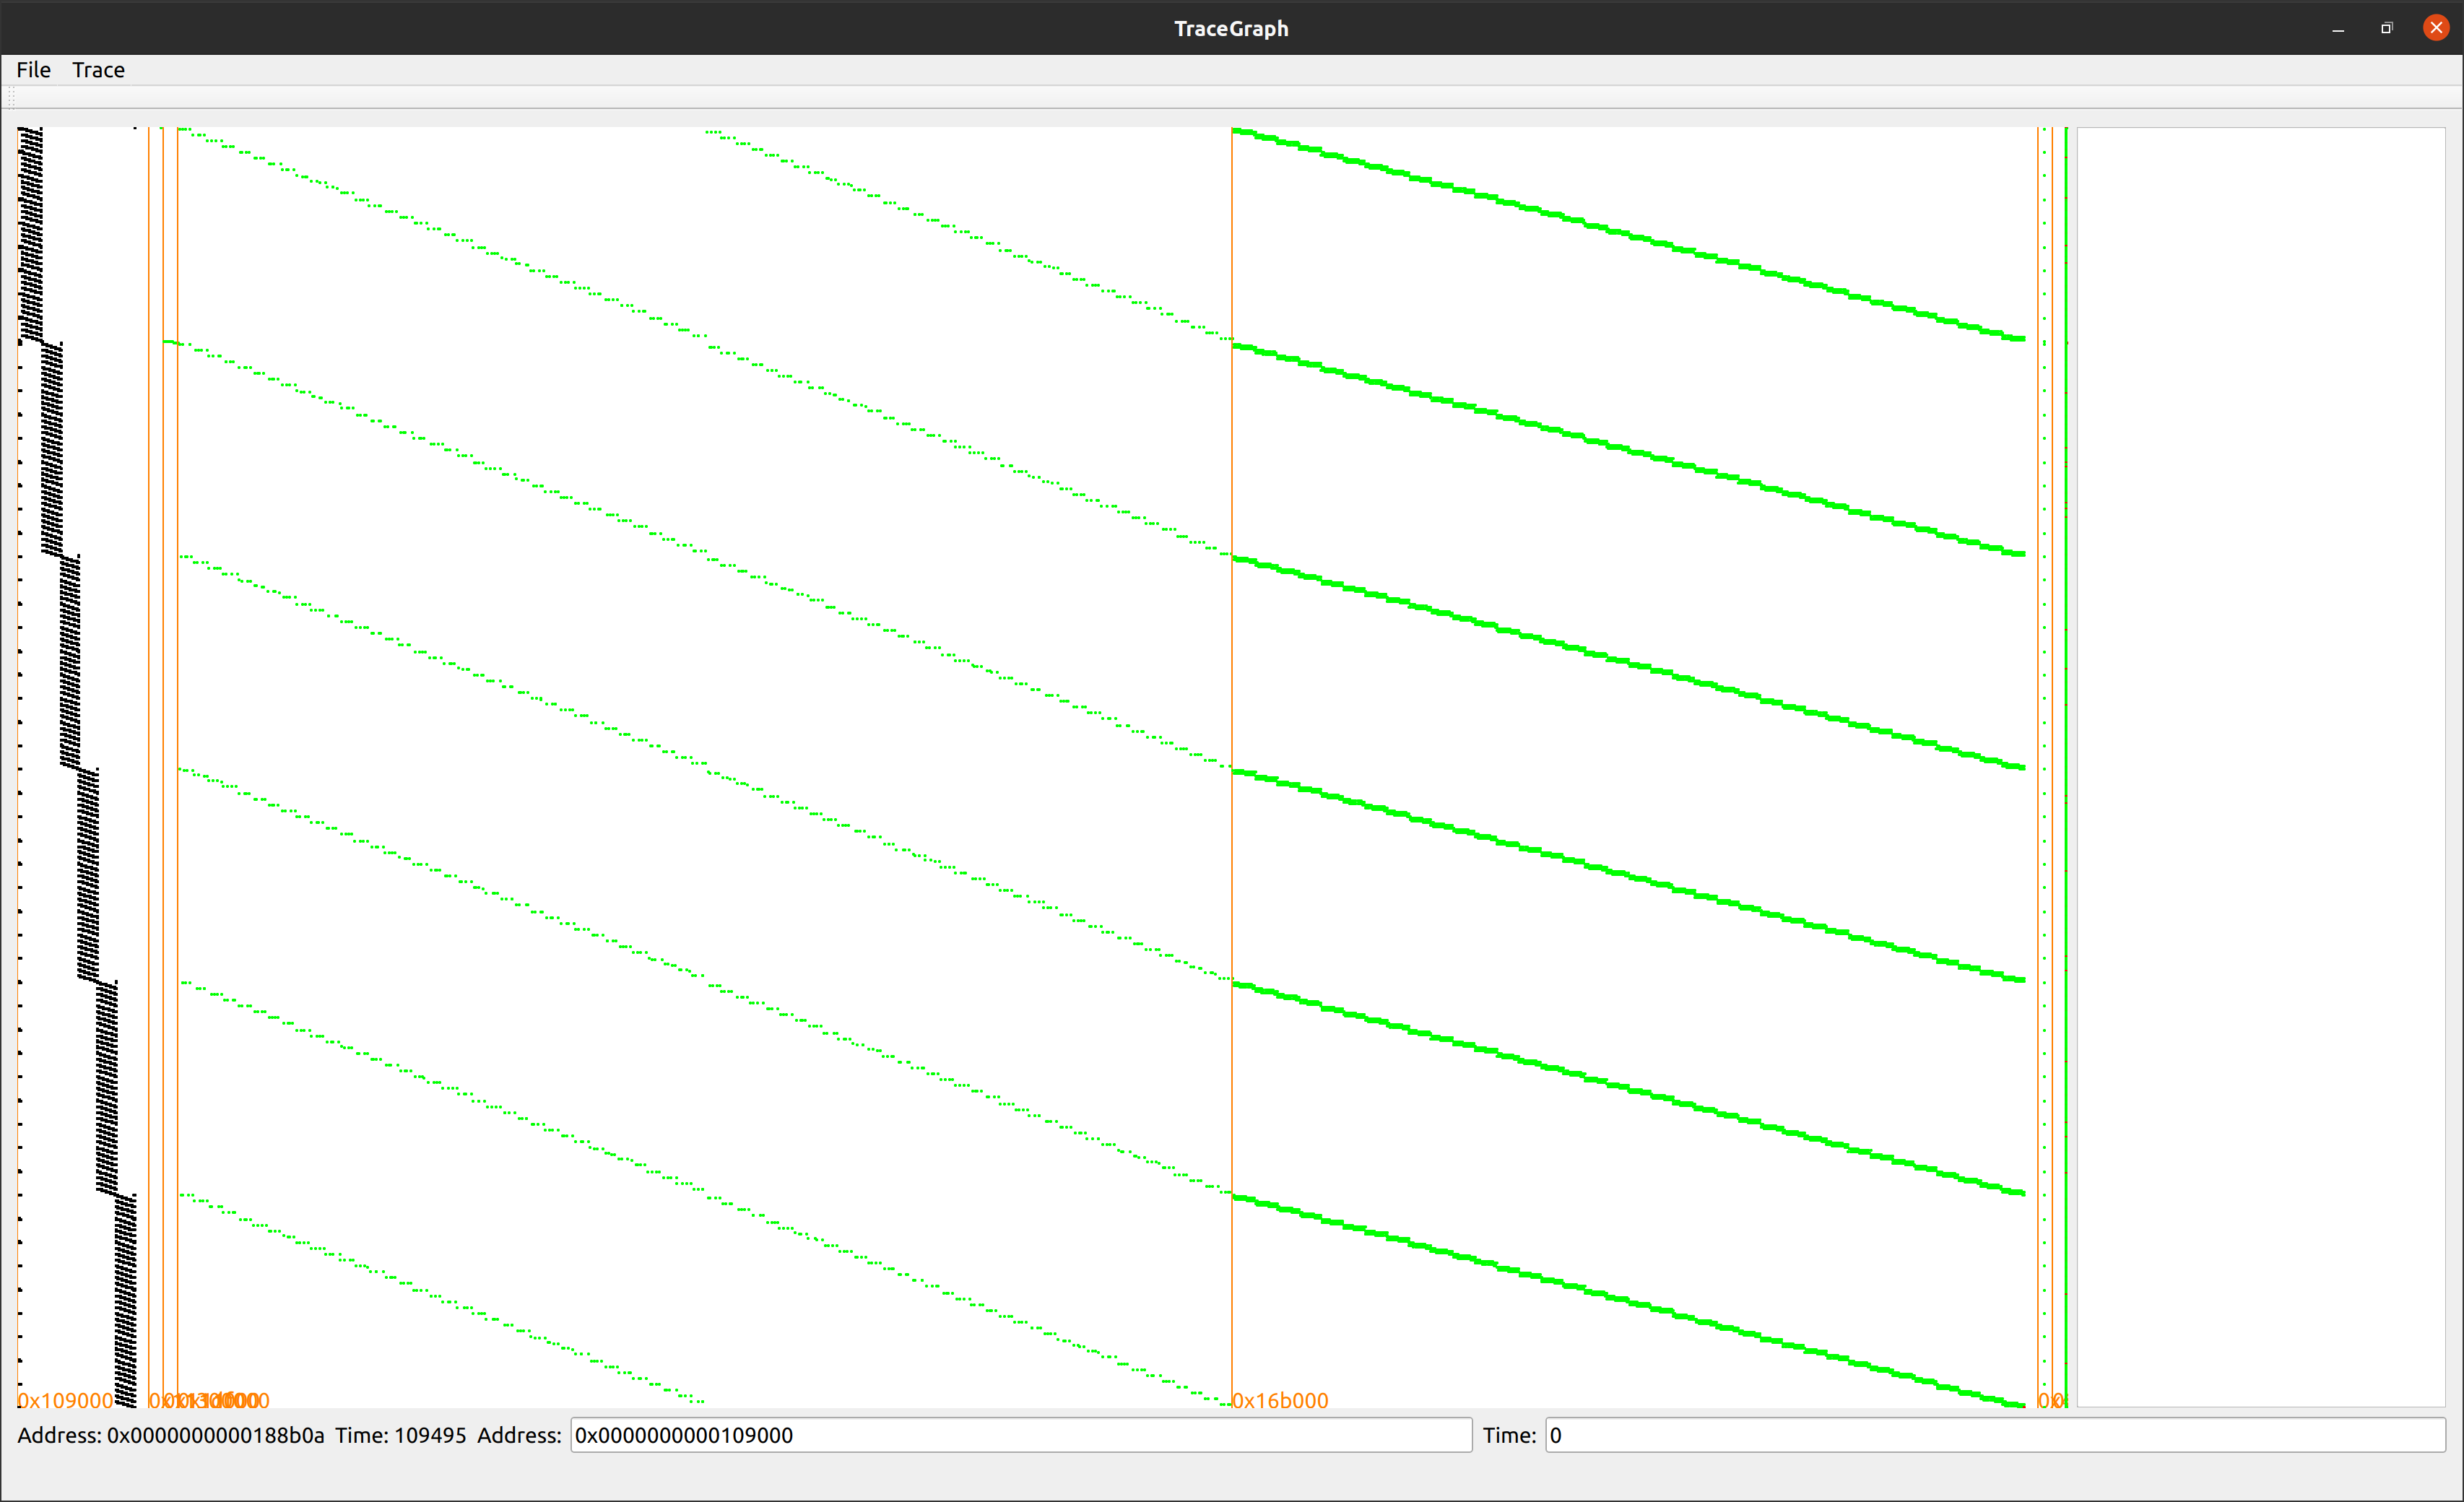
\includegraphics[scale=0.11]{Images/26_avec_filtre.png}\\
\end{center}
On génère pour commencer 30 traces avec ce filtre et on lance daredevil sur les adresses mémoire en ciblant $AES\_AFTER\_MULTINV$. On obtient 4 résultats différents pour les différents octets :\\

\begin{itemize}
\item Cas 1 :\\
\begin{center}
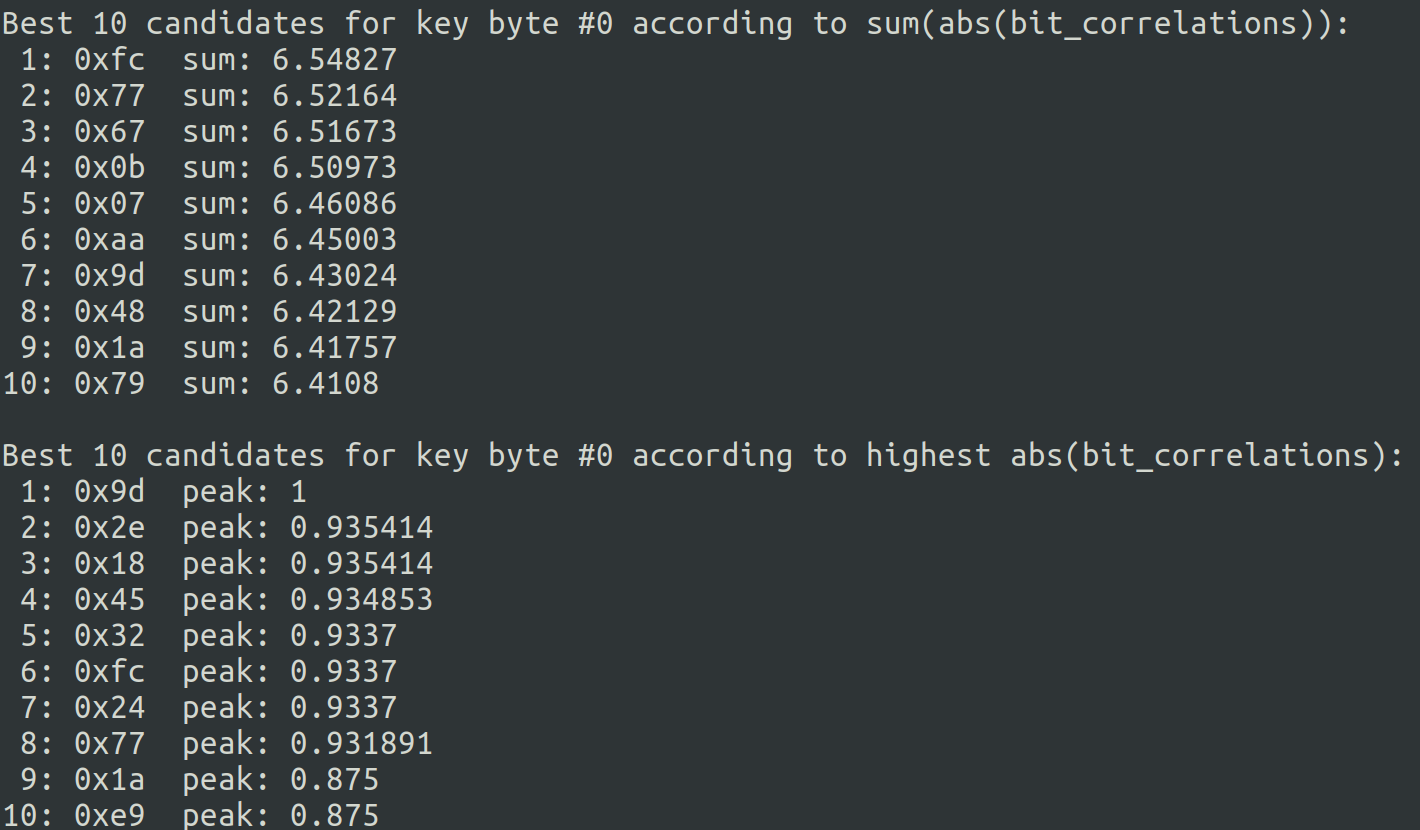
\includegraphics[scale=0.25]{Images/Resultat_26_cas_1}\\
Quand on regarde la somme des valeurs absolues de la corrélation on ne distingue pas une valeur se distinguant des autres alors que lorsqu'on regarde la valeur absolue de la corrélation, on observe qu'un octet pourrait bien correspondre.
\end{center}

\item Cas 2 :\\
\begin{center}
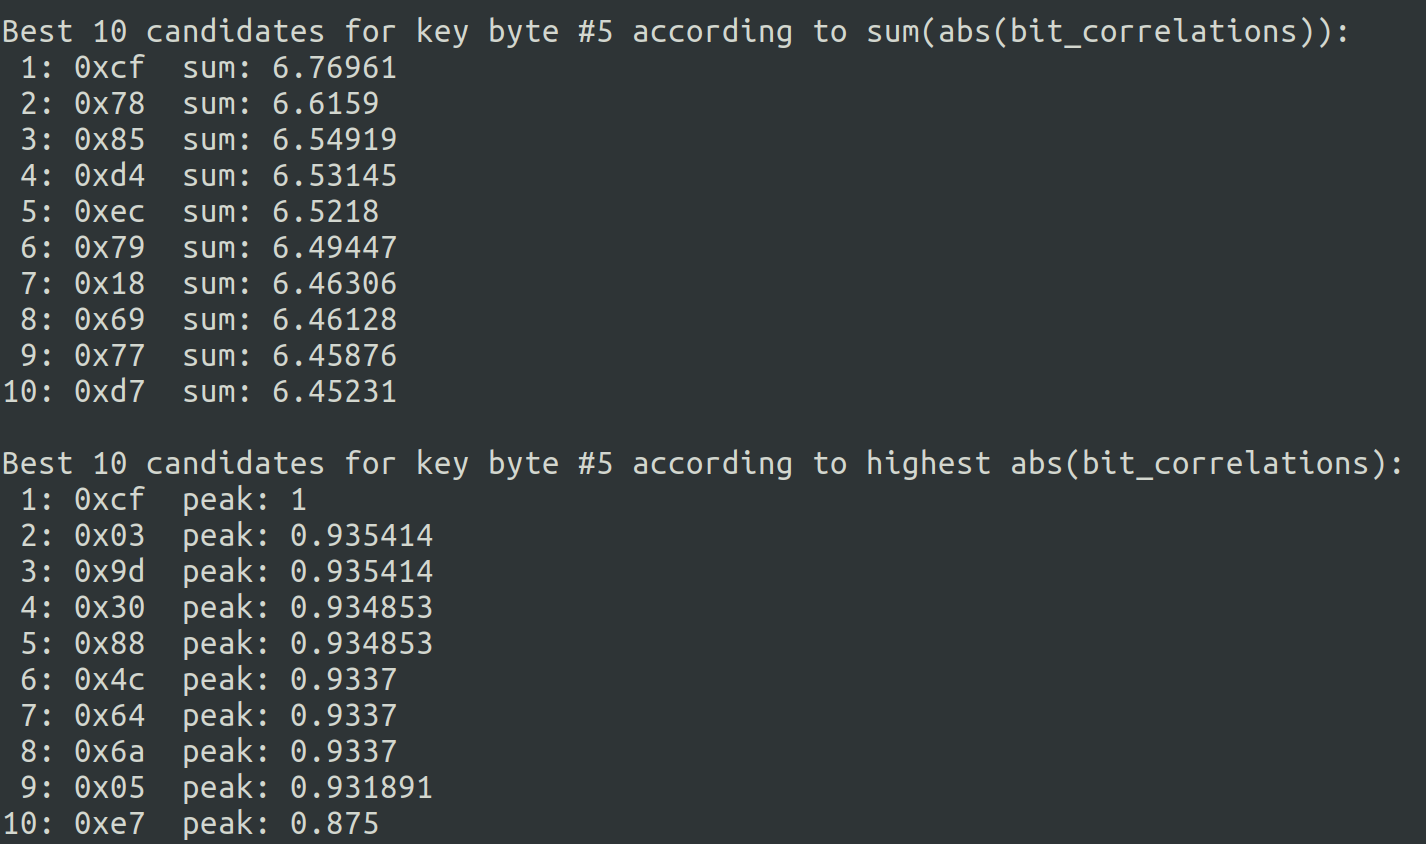
\includegraphics[scale=0.25]{Images/Resultat_26_cas_2}\\
On remarque la même chose que pour le cas précédent sauf que le "meilleur" octet indiqué par la somme des valeurs absolues est le même que celui indiqué par la valeur absolue.
\end{center}

\item Cas 3 :\\
\begin{center}
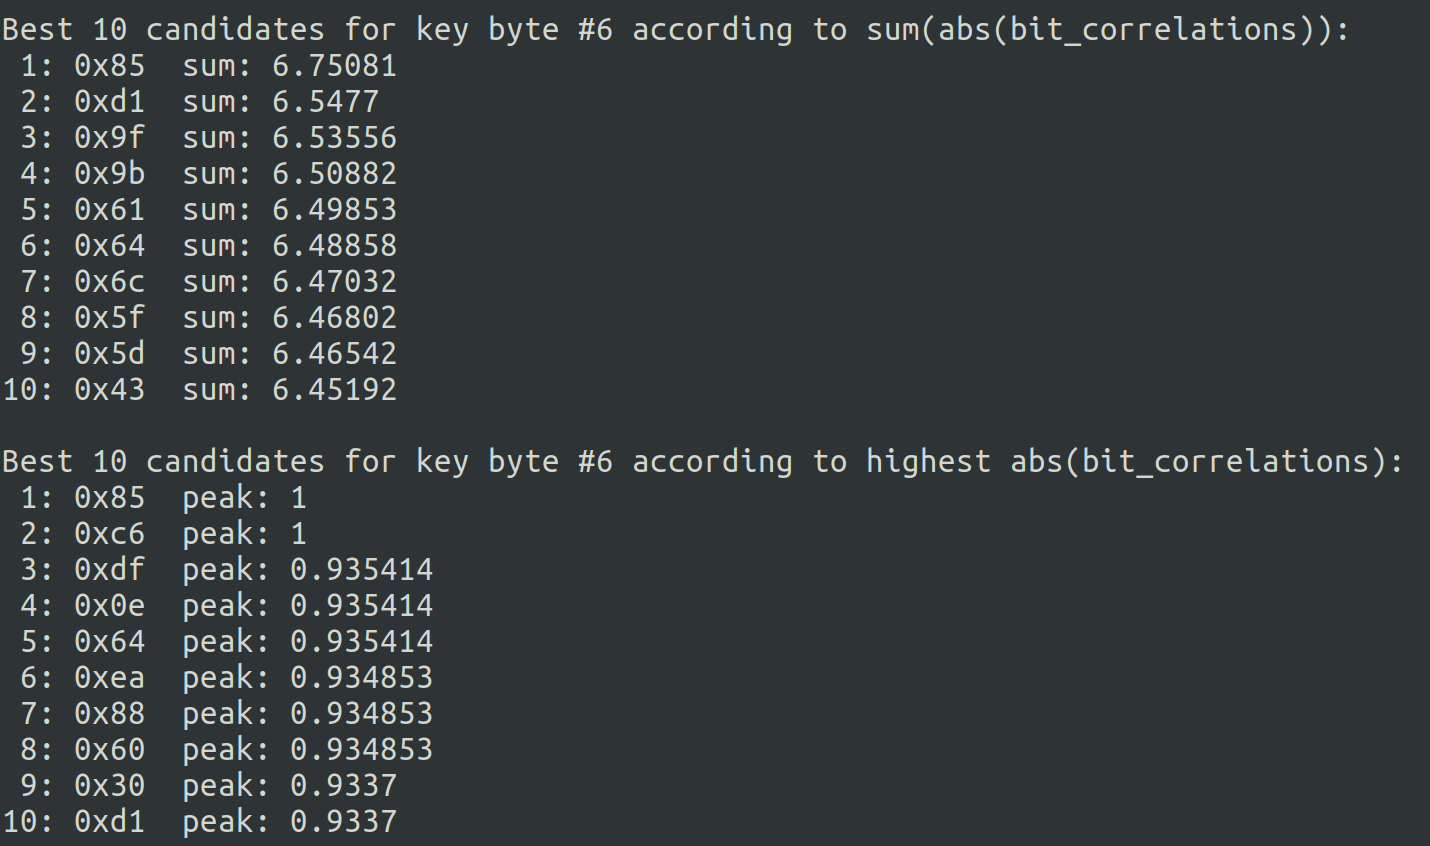
\includegraphics[scale=0.25]{Images/Resultat_26_cas_3}\\
On remarque la même chose que pour le cas précédent sauf que les deux meilleurs octets pour la valeur absolue, ont la même valeur. 
\end{center}

\item Cas 4 :\\
\begin{center}
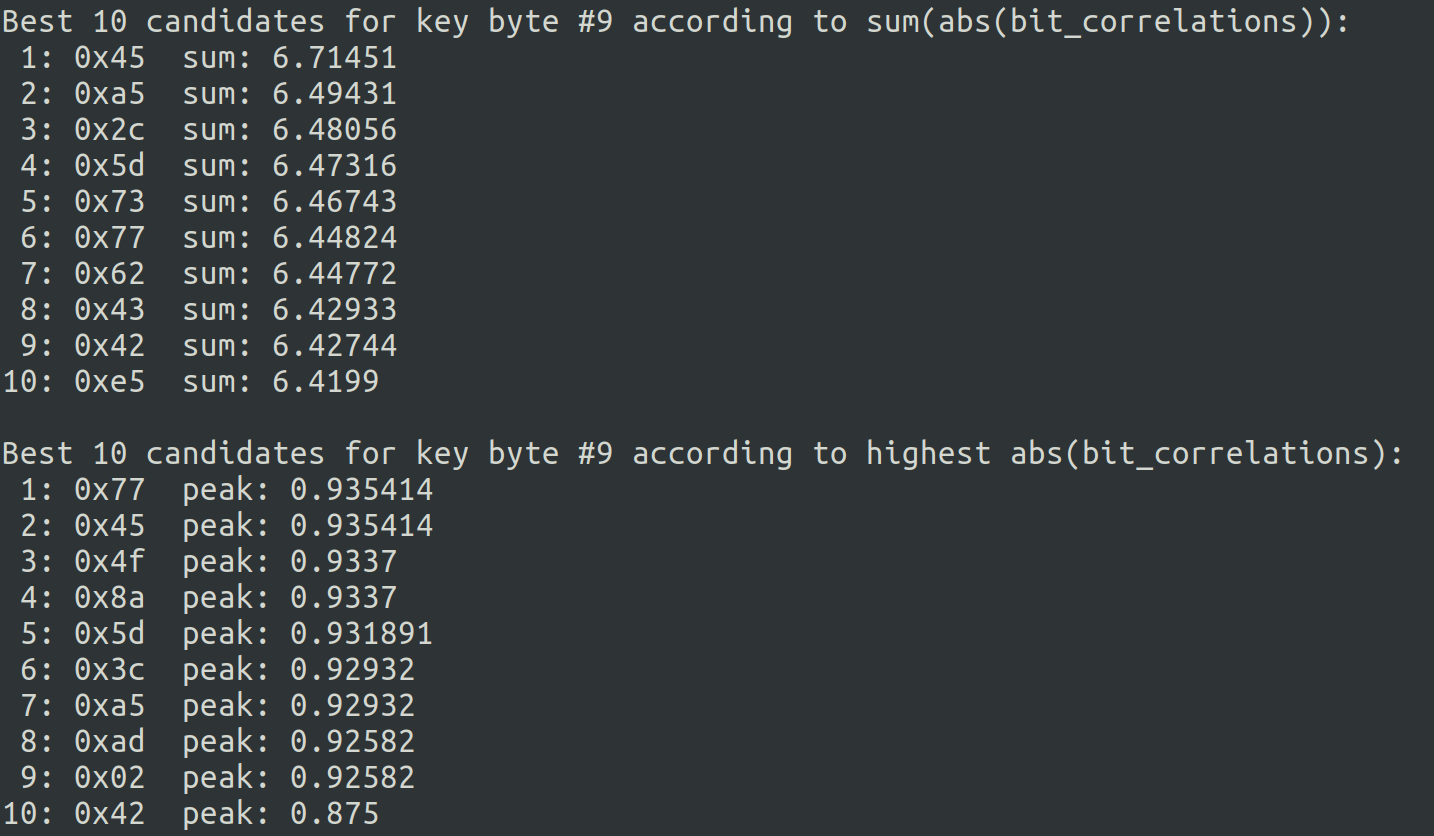
\includegraphics[scale=0.25]{Images/Resultat_26_cas_4}\\
Dans ce cas la valeur $0x45$ pourrait bien correspondre mais il est difficile d'en être sûr car l'écart entre les valeurs n'est pas très marqué.\\
\end{center}
\end{itemize}
\vspace{\baselineskip}
On peut donc noter la clé potentielle que nous avons obtenu et marquer les octets dont nous ne sommes pas certain. On relance alors plusieurs fois daredevil en changeant la position et le type de donnée que nous attaquons (adresses mémoire, données contenues aux adresses et données de la pile). On croise les différents résultats obtenus et on obtient la clé : $9D797E44B9CF850B21??8406??E3??4E$.  Les $??$ correspondent aux octets que nous n'avons pas déterminés.\\
On essaye alors de refaire la même chose mais en augmentant le nombre de traces. Je n'ai pas réussi à obtenir plus de résultat en augmentant le nombre de traces (je suis allé jusqu'à 200 traces). Comme il ne manque que 3 octets à déterminer, j'ai écrit un programme me permettant de faire une recherche exhaustive sur certains octets. Ainsi j'ai pu retrouver la clé complète étant : $9D797E44B9CF850B21DD8406FCE3AC4E$.

\subsubsection{WhibOx Contest 2017 numéro 748}
L'implémentation 748 "hungry$\_$bardeen" du WhibOx Contest de 2017 a été intéressante car elle a soulevé un problème que je n'ai malheureusement pas réussi à résoudre.\\
Tout d'abord j'ai suivi la même première étape que pour les implémentations précédentes : générer une trace complète et l'afficher pour déterminer dans quel espace se déroule l'AES. Voici ce qu'on obtient :

\begin{center}
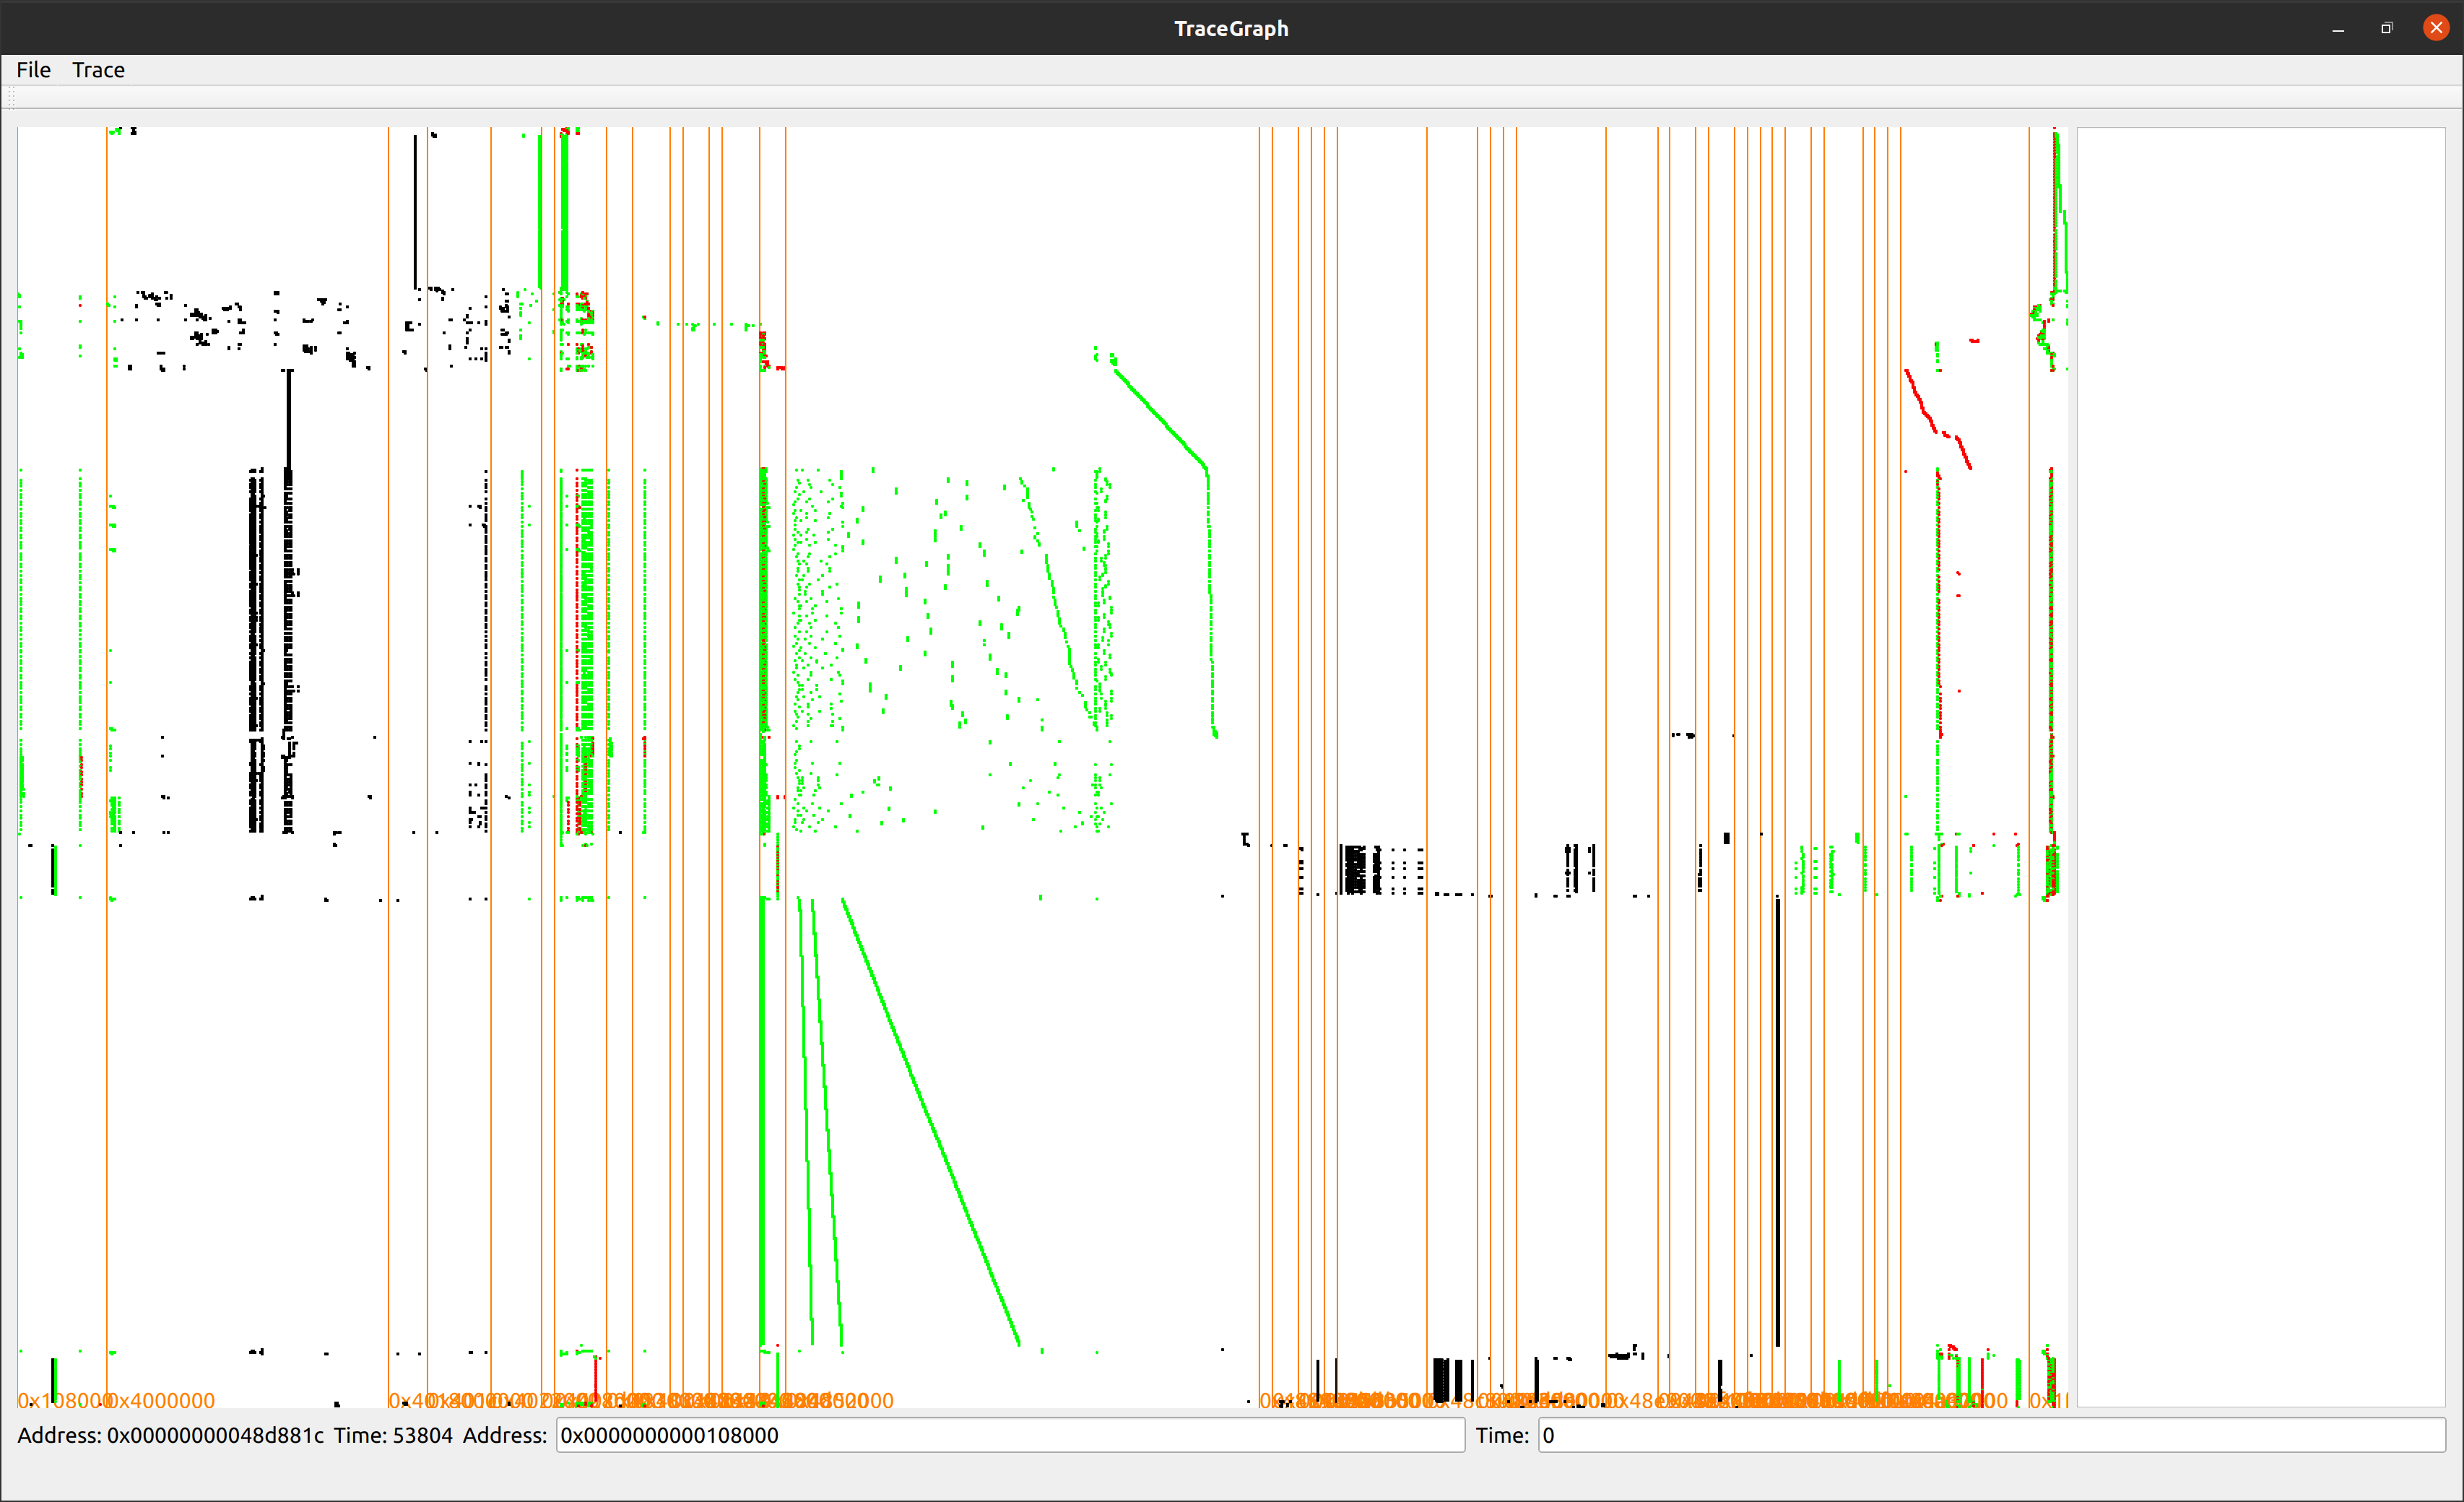
\includegraphics[scale=0.11]{Images/748_sans_filtre.png}\\
\end{center}
On ne remarque à priori rien qui pourrait ressembler à l'AES.\\
\textbf{Remarque :} Certains motifs sont toujours présents pour tous les enregistrements de traces. Il s'agit, pour la plupart, des chargements des différentes librairies système nécessaire à l'exécution.\\
J'ai alors filtré l'adresse sur l'espace $0x108000-0x4000000$ correspondant généralement à l'espace dans lequel se trouve le déroulement de l'AES (au vu de certaines autres implémentations) :

\begin{center}
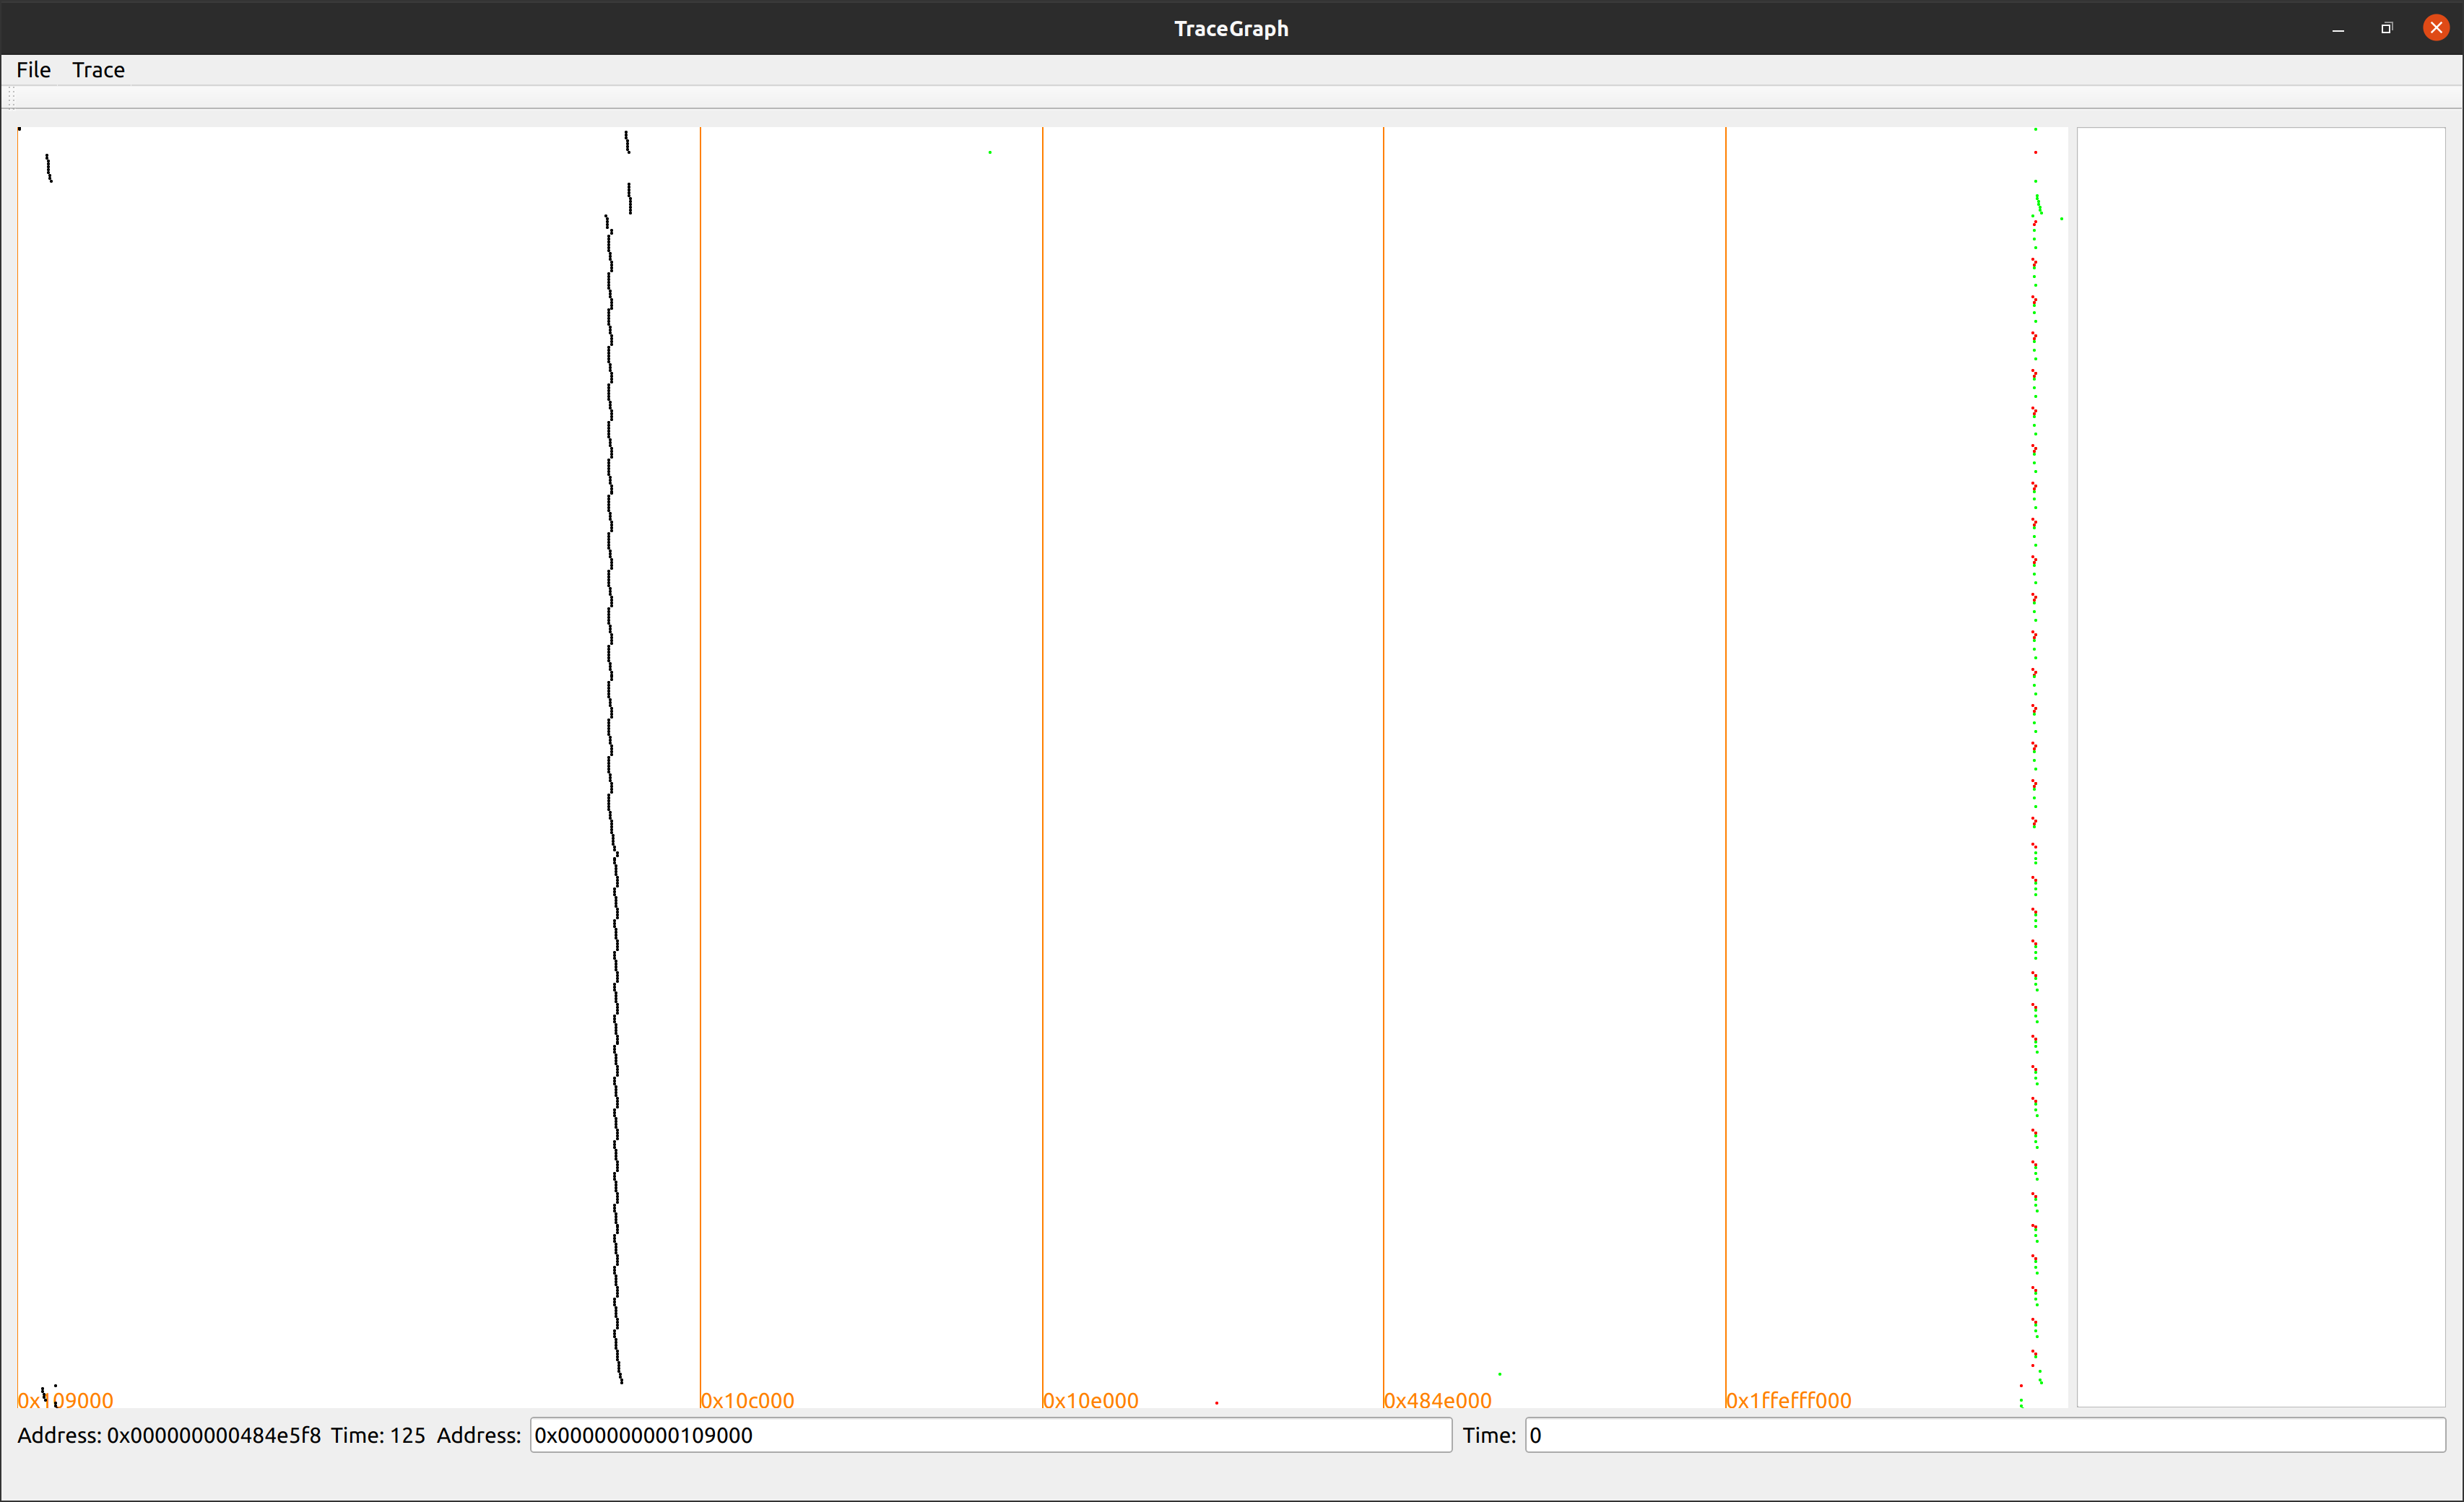
\includegraphics[scale=0.11]{Images/748_avec_filtre.png}\\
\end{center}
On observe que c'est très pauvre en terme de quantité de lecture et d'écriture comparé aux autres implémentations. Je lance quand même daredevil avec 200 enregistrements différents (filtrés avec ce filtre) mais je n'obtient aucun résultat intéressant. Suite à ça je me suis penché plus sur la trace complète et j'ai essayé de comprendre mieux comment l'implémentation fonctionnait en regardant le code source mais je rien réussi à en déduire.\\
Je décide de lancer l'enregistrement de 200 traces mémoire mais cette fois ci sans filtres ce qui rend l'attaque moins précise et moins efficace mais au moins me permet de tout englober. En lançant daredevil sur les données contenues dans les différentes adresses, on n'obtient, pour quasiment tous les octets, aucun résultat se démarquant réellement des autres. 1 ou 2 octets cependant ont l'air d'avoir un score un peu meilleur. Je répète alors la même chose mais cette fois ci avec 1000 enregistrements. On obtient le même genre de résultat que précédemment. Et pareillement avec 2000.\\
J'ai rencontré ce problème sur plusieurs implémentations.


\subsubsection{WhibOx Contest 2017 numéro 777}
L'implémentation 777 "adoring$\_$poitras" du WhibOx Contest de 2017 m'a elle aussi posé un problème que j'ai rencontré sur plusieurs implémentations : lorsque je lance l'enregistrement d'une trace mémoire, l'enregistrement ne s'arrête jamais. J'ai longtemps essayé de résoudre ce problème par différents moyens notamment en essayant de paramétrer Valgrind d'une autre manière, en utilisant TracePin et en rajoutant de la puissance à ma machine virtuel mais cela n'a donné aucun résultat.\\
J'ai essayé plus tard de forcer l'exécution de l'AES à se stopper en ajoutant un processus dans ma fonction $main()$ et en ajoutant un timer : le processus père attend un certain nombre de secondes et tue le processus fils exécutant l'AES. La trace mémoire n'est donc pas complète, cependant comme daredevil n'attaque que sur le premier tour de l'AES, on peut espérer que le premier tour s'est au moins déroulé. Le chiffré en sortie devient également erroné mais ce n'est pas un problème car daredevil n'as pas besoin d'utiliser les messages de sorti de l'AES pour effectuer la CPA.\\
Voici ce qu'on obtient :

\begin{center}
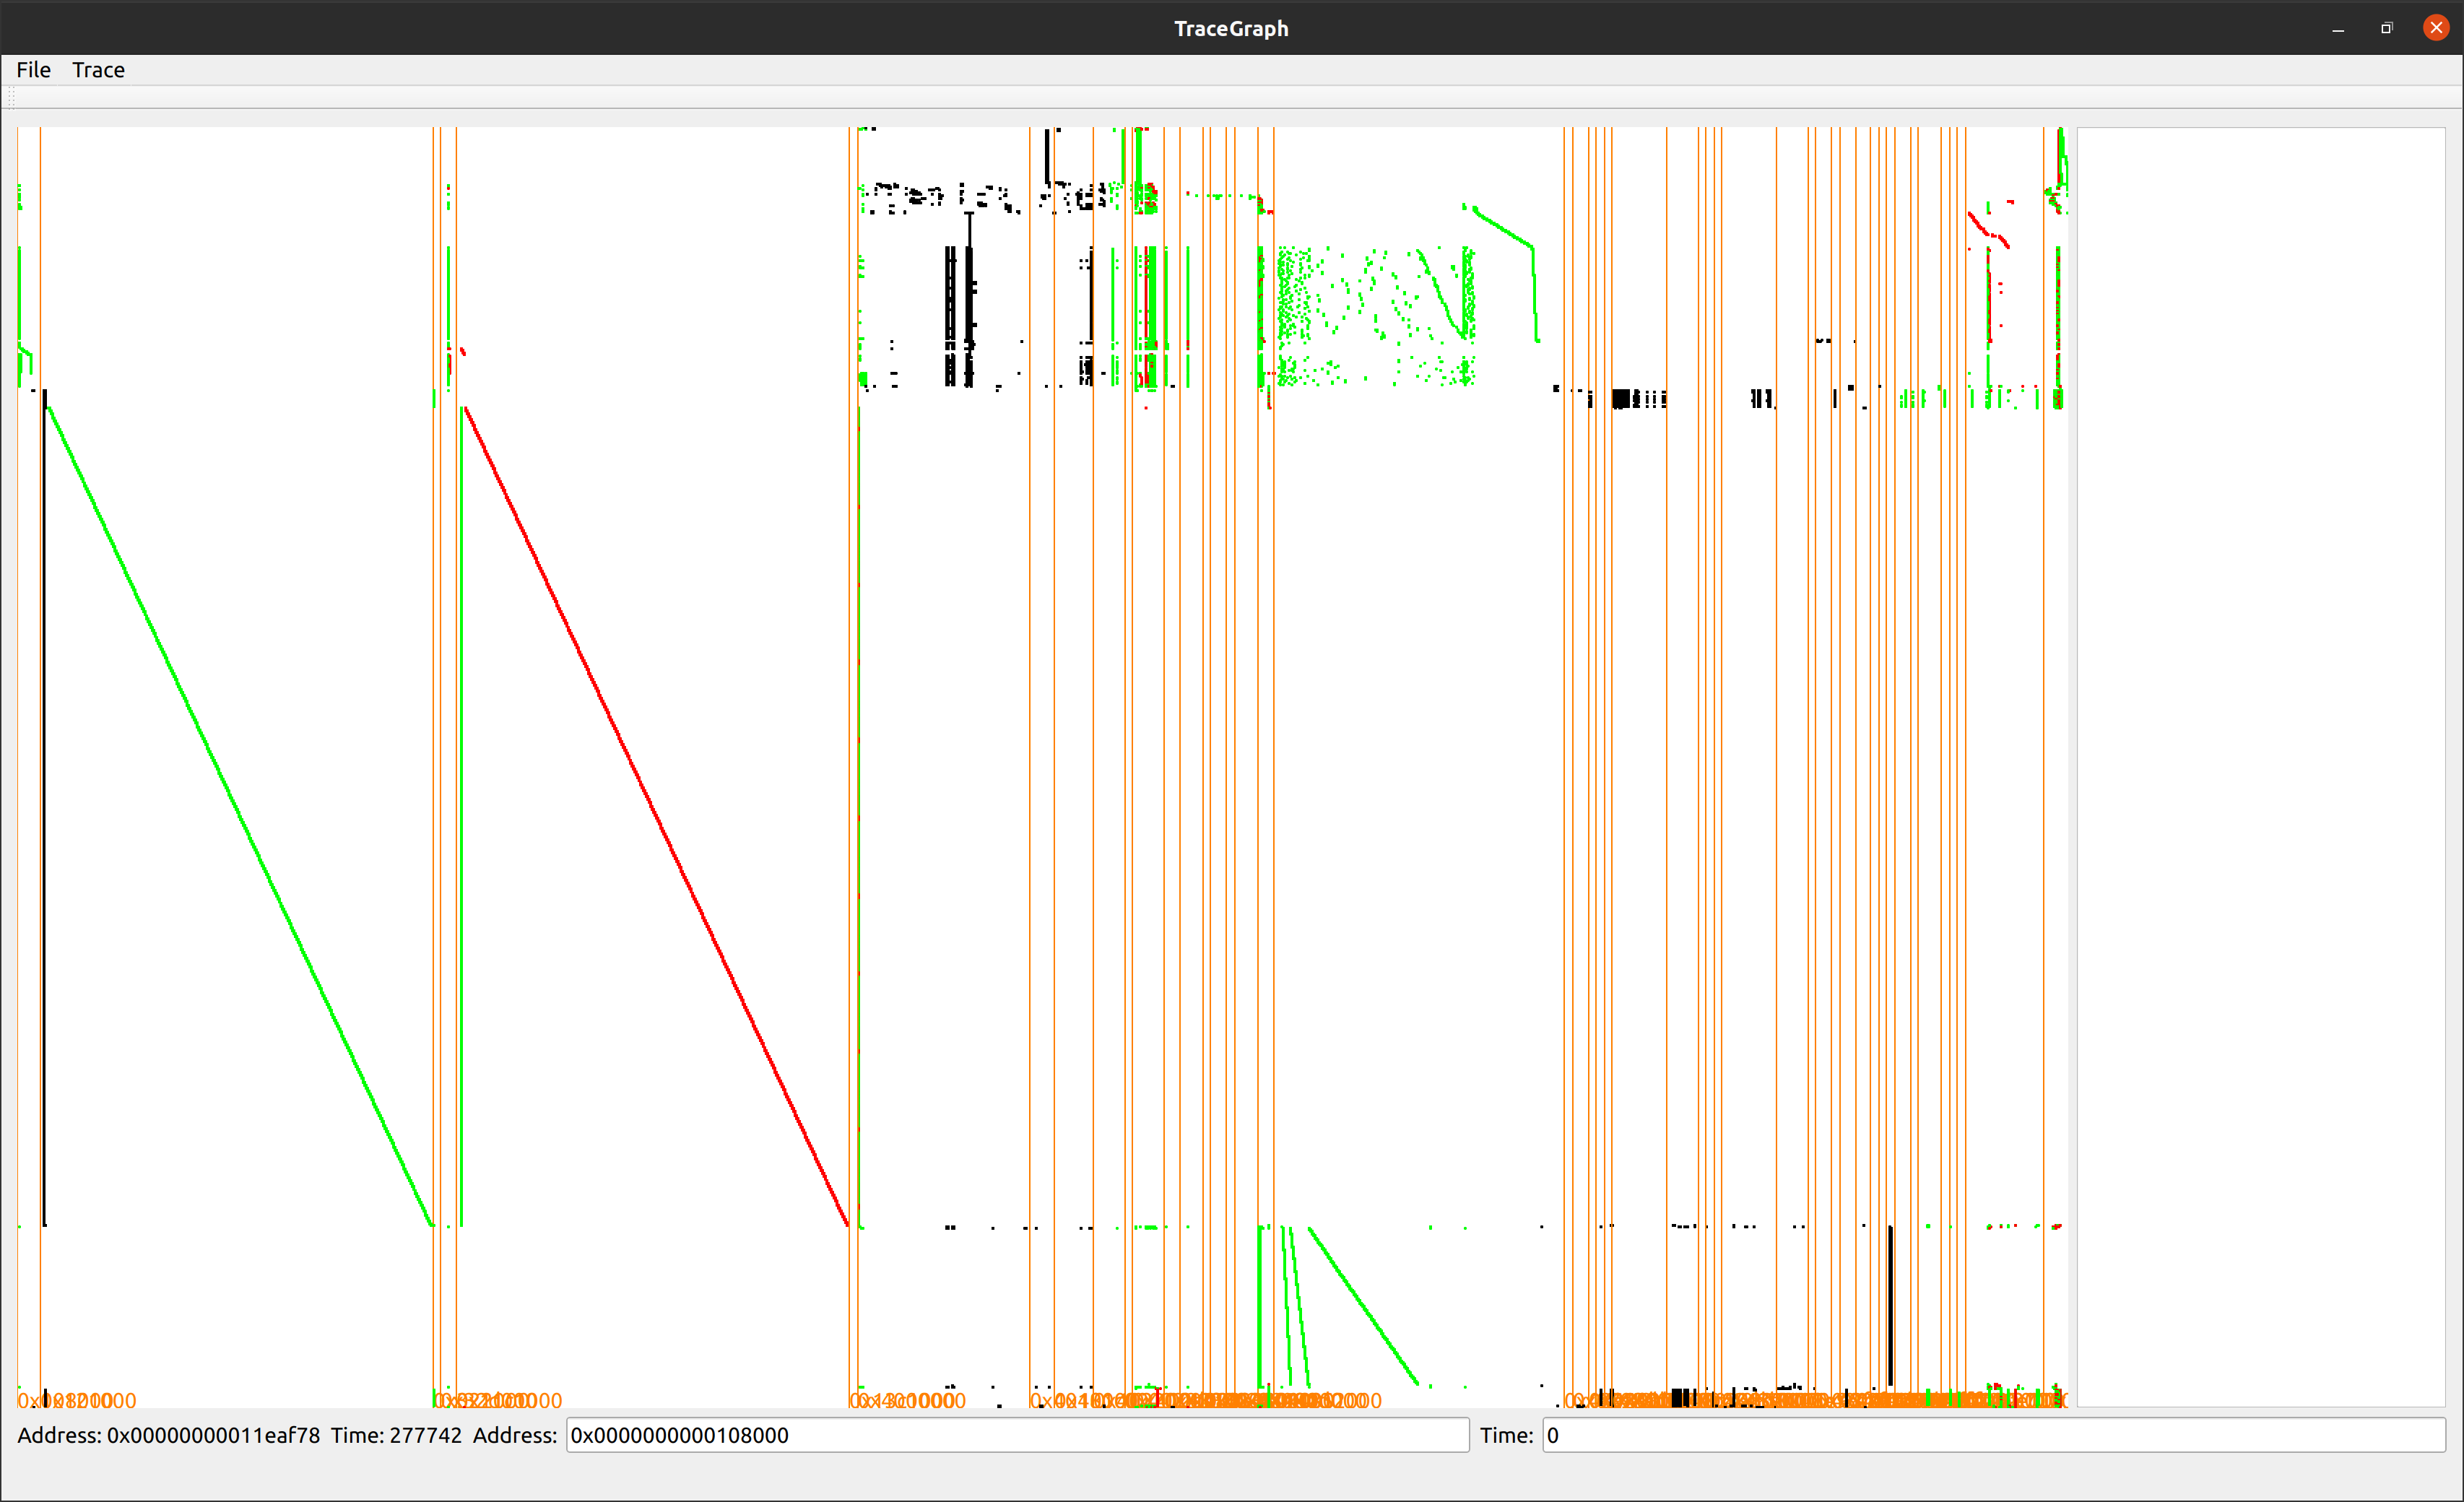
\includegraphics[scale=0.11]{Images/777_sans_filtre.png}\\
\end{center}
On remarque clairement un motif inhabituel prenant la plus grande place dans cette trace mémoire.
On lance l'enregistrement de 100 traces pour commencer et on exécute daredevil avec les différentes configurations possibles. On obtient le même genre de résultat que pour l'implémentation précédente : aucune déduction possible sur les différents octets de clé sauf quelques suspicions pour certains. On essaye cette fois ci de lancer une attaque d'ordre 2 (dans le cas où il y aurait un masquage d'ordre 2) avec différents paramètres mais on n'obtient rien non plus.\\
On décide d'augmenter le nombre de traces à 200 et cette fois ci. Aucun résultat ne se distingue et rien ne va dans le sens des suspicions faites pour 100 traces. Pareillement pour 800 traces.\\
J'ai essayé longtemps plusieurs configurations possible mais je ne suis pas arrivé à trouver la clé pour cette implémentation.\\
La solution étant peut être d'augmenter encore le nombre de traces, cependant l'enregistrement de 800 traces et l'exécution de daredevil pour cette implémentation était déjà très long.\\
J'ai retravaillé sur cette implémentation un peu plus tard et ait constaté quelque chose dont je ne m'étais pas aperçu initialement : le formatage automatique des traces avec deadpool ne se faisait pas bien. Deadpool considérait que la taille des données à analyser était de 4 octets alors qu'en réalité elle était de 8 octets. Ceci était dû au fait que j'utilisais les filtres par défaut proposés par deadpool pour le formatage. J'ai donc relancé l'acquisition de traces en spécifiant les filtres à utiliser pour le formatage (la variable $filters$ en paramètre de la classe $TracerGrind$ et la variable $keywords$ en paramètre de la fonction $bin2daredevil$) toujours en forçant l'arrêt de l'exécution au bout d'une seconde. Cela n'a malheureusement pas donné de résultats exploitables après le lancement de daredevil pour 100 traces. Je n'ai pas essayé avec plus de traces car l'analyse était déjà très longue (environ 18 minutes par octet).


\subsection{Implémentation de Rivain-Prouff avec masquage d'ordre 1}
Il est possible de trouver sur le dépôt \href{https://github.com/coron/htable}{https://github.com/coron/htable} plusieurs implémentations du DES et de l'AES utilisant différentes contremesure. Ici je me suis intéressé à l'implémentation utilisant la contremesure de Rivain-Prouff avec un masquage d'ordre 1.\\
On commence par générer une trace complète :

\begin{center}
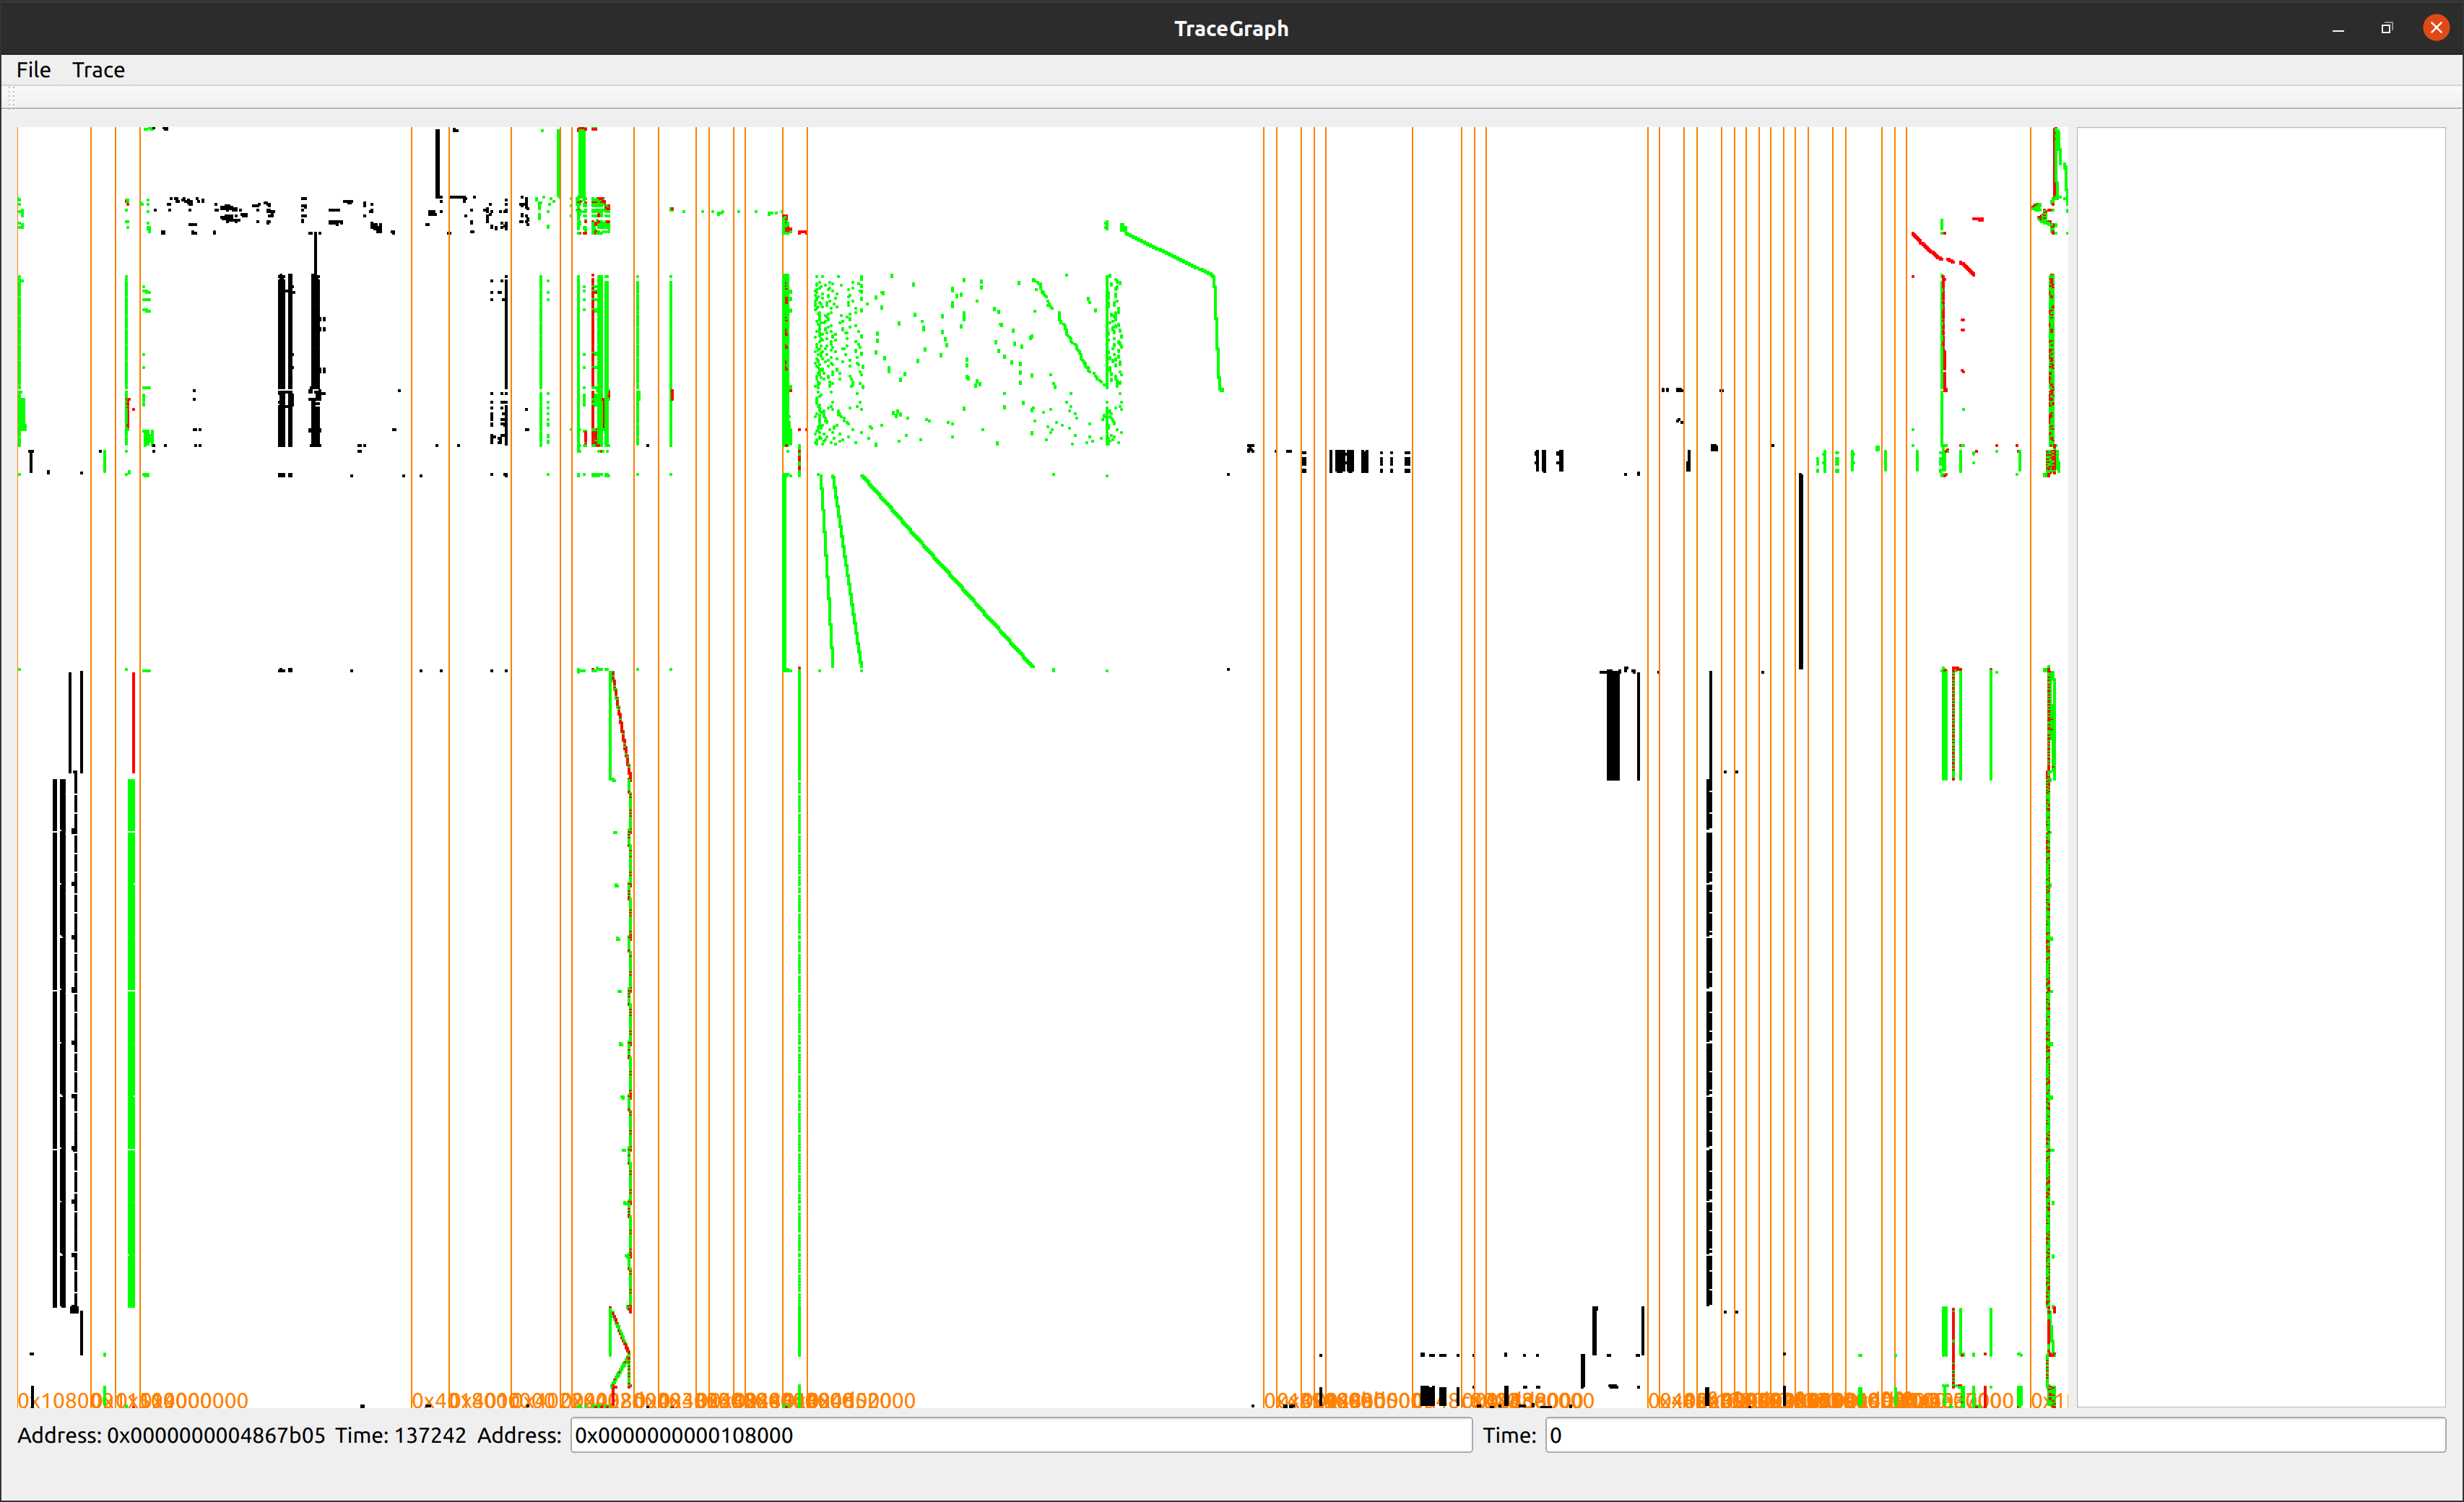
\includegraphics[scale=0.11]{Images/Rivain_Prouff_sans_filtre.png}\\
\end{center}
On reconnait assez bien le motif de l'AES :

\begin{center}
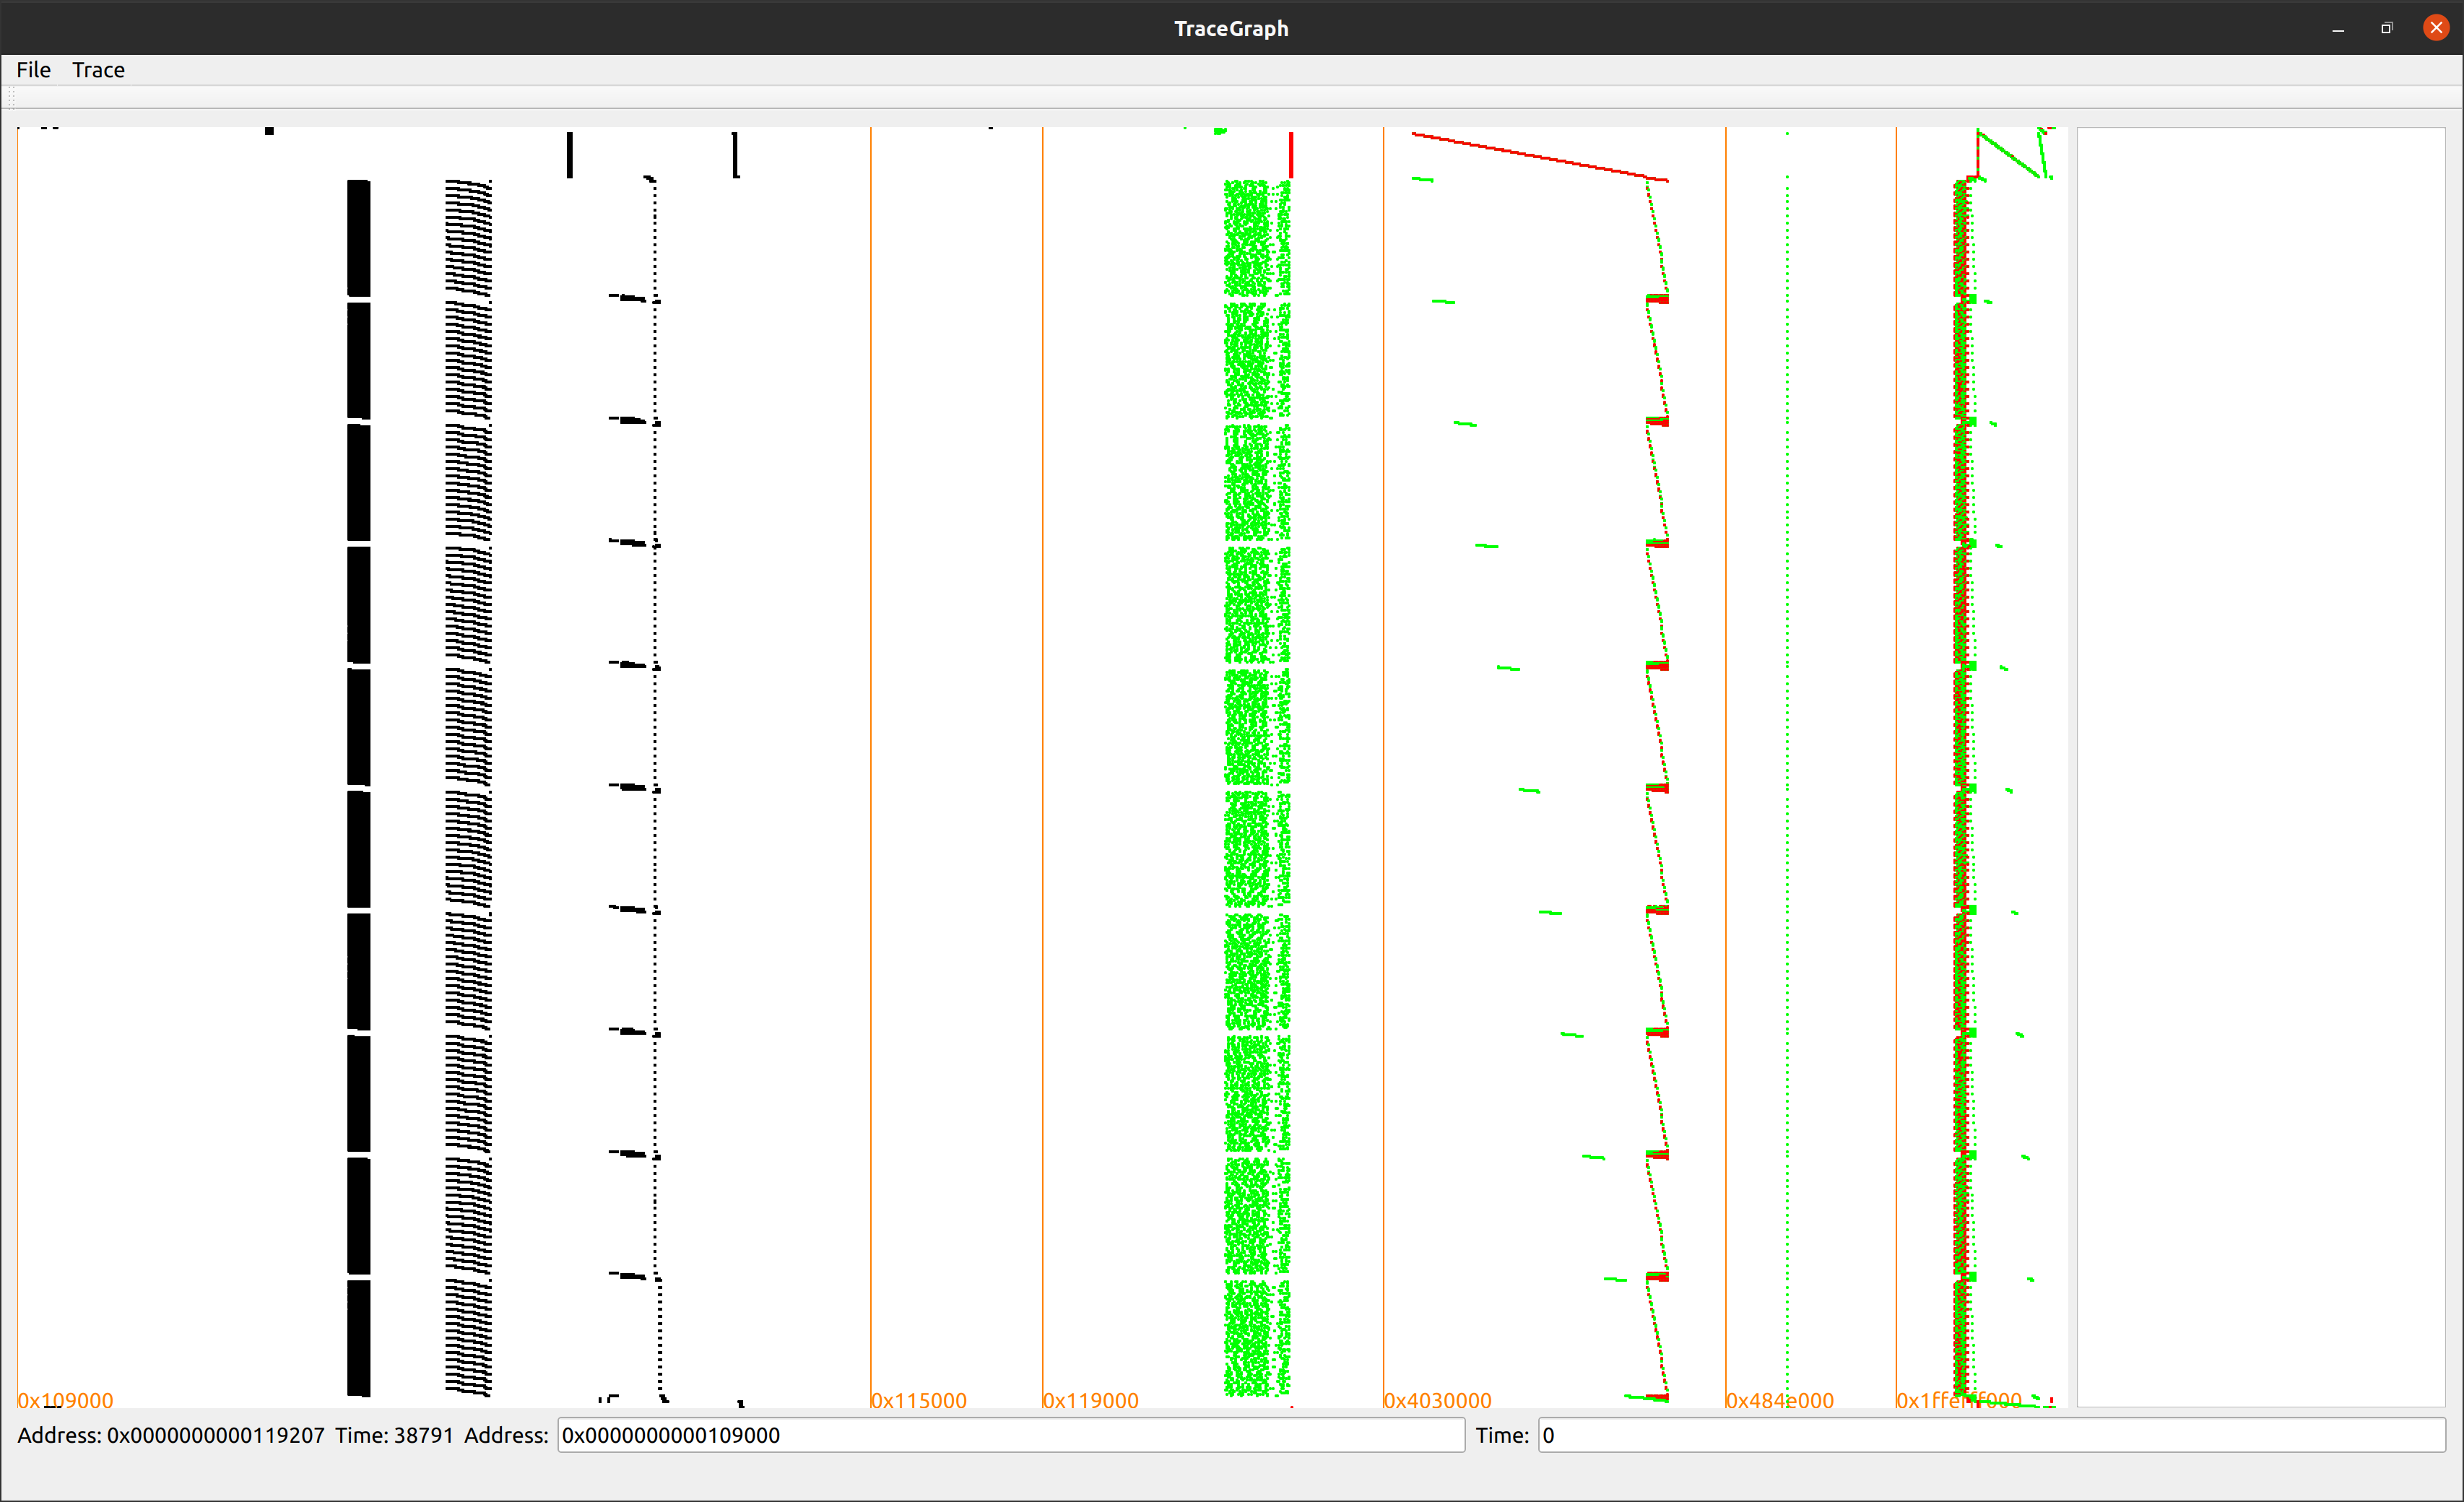
\includegraphics[scale=0.11]{Images/Rivain_Prouff_avec_filtre.png}\\
\end{center}
On lance alors l'enregistrement de 100 traces avec les filtres mémoire couvrant toute la zone dans laquelle l'AES se déroule. On lance une CPA d'ordre 1 avec daredevil et on obtient aucune information sur les octets de clé. On essaye en utilisant plusieurs positions différentes et plusieurs types de données différents et le résultat reste le même. Ceci est cohérent car l'attaque est d'ordre 1 alors que l'implémentation contient un masquage d'ordre 1.\\
On essaye maintenant en changeant les fichiers de configuration : On met la variable $order$ à 2 et la variable $window$ à 10 pour commencer. Voici comment se présente le résultat :

\begin{center}
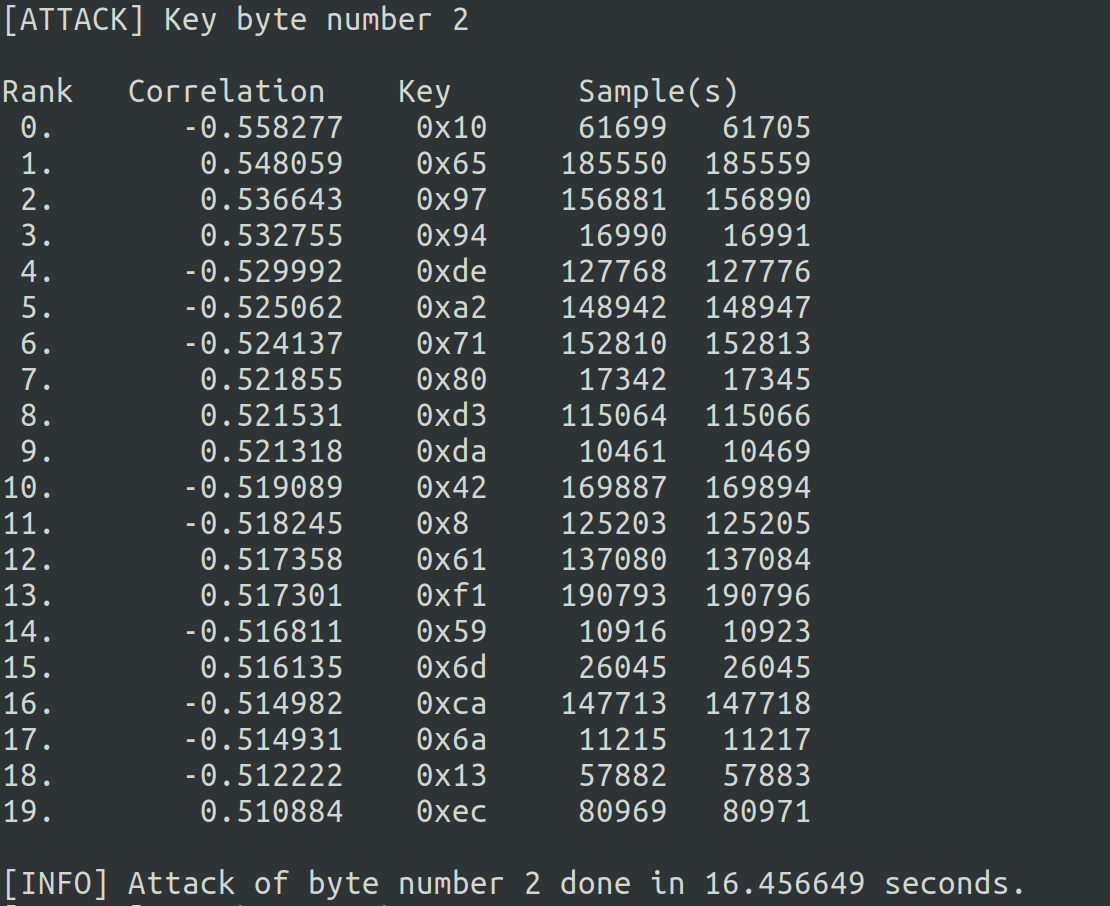
\includegraphics[scale=0.30]{Images/Rivain_Prouff_ordre_2.png}\\
\end{center}

Aucun résultat ne semble se démarquer. L'idée initiale était que cette "fenêtre" d'analyse (donnée par la variable $window$) n'était pas suffisante. On relance alors daredevil plusieurs fois avec les même traces en augmentant progressivement la variable $window$. Cela n'amène pas de résultat positif et on remarque que le temps de l'analyse augmente considérablement lorsqu'on incrémente cette variable. Voici la liste des choses faites pour tenter d'obtenir un résultat :

\begin{itemize}
\item Augmenter le nombre de trace
\item Diminuer le nombre de sample à analyser (essayer de cibler plus précisément le premier tour de l'AES)
\item Augmenter la taille de la fenêtre
\item Comme on avait accès au code source, restreindre l'exécution de l'AES à l'exécution du premier tour et ainsi obtenir des fichiers de trace moins volumineux\\
\end{itemize}
Finalement en "jouant" avec tous ces paramètres tout en gardant une durée de l'attaque faisable, je n'ai eu aucun résultat positif.\\
Je me suis penché alors plus particulièrement sur la compréhension de ce que faisait daredevil lors d'une CPA du second ordre. J'ai eu, pendant un moment, plusieurs incompréhension concernant la validité du code mais finalement, il me semble bien correct dans ce qu'il fait.\\
Une autre solution serait peut-être d'augmenter considérable la variable $window$ et le nombre de traces par rapport à ce que j'ai fait. Je n'ait donc pas réussi à trouver la clé pour cette implémentation.


\section{Liens Utiles}

\begin{itemize}
\item Utilisation et explication des outils de SideChannelMarvels et attaques par DCA par les créateurs des outils de SideChannelMarvels :\\
\url{https://www.sstic.org/media/SSTIC2016/SSTIC-actes/design_de_cryptographie_white-box_et_a_la_fin_c_es/SSTIC2016-Article-design_de_cryptographie_white-box_et_a_la_fin_c_est_kerckhoffs_qui_gagne-hubain_teuwen_1.pdf}\\

\item Cryptanalyse sur les implémentations en boîte blanche de l'AES :\\
\url{https://link.springer.com/content/pdf/10.1007\%2F978-3-540-30564-4_16.pdf}\\

\item Passer outre un encodage affine sur une implémentation en boîte blanche :\\
\url{https://eprint.iacr.org/2019/096.pdf}\\

\item Attaques et contremesures sur les conceptions en boîte blanche (notamment avec masquage) :\\
\url{https://eprint.iacr.org/2018/049.pdf}\\

\item Contre-mesure contre les DCA d'ordre supérieur à 1 :\\
\url{https://eprint.iacr.org/2010/523.pdf}\\
\url{https://link.springer.com/content/pdf/10.1007\%2F978-3-642-15031-9_28.pdf}\\

\item Attaques sur l'implémentation \textit{adoring poitras} :\\
\url{https://eprint.iacr.org/2018/098.pdf}\\

\item Mon dépôt GitHub regroupant les attaques (ou tentatives d'attaques) décrites dans ce récapitulatif :\\
\url{https://github.com/jeandestribois/Stage_2020}\\
\end{itemize}


\end{document}